%%%%%%%%%%%%%%%%%%%%%%%%%%%%%%%%%%%%%%%%%%%%%%%%%%%
%
%  New template code for TAMU Theses and Dissertations starting Fall 2012.  
%  For more info about this template or the 
%  TAMU LaTeX User's Group, see http://www.howdy.me/.
%
%  Author: Wendy Lynn Turner 
%	 Version 1.0 
%  Last updated 8/5/2012
%
%%%%%%%%%%%%%%%%%%%%%%%%%%%%%%%%%%%%%%%%%%%%%%%%%%%

%%%%%%%%%%%%%%%%%%%%%%%%%%%%%%%%%%%%%%%%%%%%%%%%%%%%%%%%%%%%%%%%%%%%%%%
%%%                           SECTION II
%%%%%%%%%%%%%%%%%%%%%%%%%%%%%%%%%%%%%%%%%%%%%%%%%%%%%%%%%%%%%%%%%%%%%%

\renewcommand*{\thefootnote}{\fnsymbol{footnote}}
\chapter[Chapter1]{\uppercase {Chapter1}\symbolfootnote[1]{Reprinted with permission from ``Introduction: The Importance of Research'' by AUTHOR et al., 2015. The Astrophysical Journal, Volume XYZ, Issue X, article id. XY, XY pp., Copyright 20XX by the American Astronomical Society.} }
\renewcommand*{\thefootnote}{\arabic{footnote}}
\setcounter{footnote}{0}

\section{Introduction}\label{sec: Introduction}
Our ability to perform precision cosmology with clusters of galaxies has reached a critical point. The widely accepted $\Lambda$CDM model of cosmology makes explicit predictions about the mass function of galaxy clusters in the universe. Measuring this mass function across many redshifts, in turn, provides constraints on the cosmology. Today, large-area sky surveys are providing observations of large numbers of clusters, but systematics in deriving cluster masses dominate the error budget \citeeg{Sehgal2011,Plank2014, Bocquet2015}. To place further constraints on the $\Lambda$CDM model of cosmology, we must decrease these systematics. 

As mass is not a direct observable, a lot of work is underway to characterize galaxy cluster masses with an observable feature of galaxy clusters. The goal is to constrain $P(M|z, \vec{x})$ the probability density ($P$) that a galaxy cluster of given mass ($M$), located at redshift ($z$) determined using an observable parameter or parameters ($\vec{x}$). Generally, cluster mass calibrations are done in one of two ways, through simulations or direct or statistical calibration.

One could use various simulations to attempt to calibrate this observable-mass relation \citeeg{Vanderlinde2010, Sehgal2011}. However, the primary challenge to this method is the incomplete understanding of the baryonic physics which take place in galaxy cluster environments. While there have been (and continue to be) many improvements in the accuracy and power of simulations it is doubtful that in the coming years they will reach the accuracy level required where the observable--mass relation is dominated only by statistics \citep{Weinberg2013}. 
 
The second broad method is the direct calibration of cluster masses. This recipe has two distinct but not always independent tracks. The ``direct'' method uses observations of a relatively small set of clusters and then uses known mass estimators, including X-ray temperatures and luminosities \citeeg{Mantz2010, Rykoff2014}, microwave observations \citeeg{Vanderlinde2010, Sehgal2011}, optical richness \citeeg{Abell1958, Rykoff2012} or weak lensing (WL; \eg\ \citealt{Rozo2010}) as examples, which provide a ``true'' mass. This directly calibrates the observable-mass relation which is then applied to a much larger sample. The complications lie in that the ``true'' masses are, in fact, estimations, and the methods used to recover these cluster masses are subject to their own limitations. X-ray based cluster masses assume hydrostatic equilibrium \citeeg{Mantz2015} which may only be valid for a very small number and range of cluster masses. The Sunyaev-Zel'dovich Effect (SZE; \citealt{Sunyaev1972}), which uses the up-scattering of cosmic microwave background (CMB) photons to estimate cluster masses, provides accurate estimations of mass, but the ability to detect low mass galaxy clusters is currently limited by technology \citeeg{Carlstrom2002a} and can also be effected by the properties of the intracluster medium \citeeg{Pipino2010}. WL estimates are, in principle, correct in the mean, but they suffer from signal-to-noise requirements, limiting their usefulness in low mass clusters (where the lensing signal is particularly weak), and potentially suffer from line-of-sight effects as WL is sensitive to all mass along the line-of-sight. Virial mass estimators which determine the cluster mass based on the motions of the member galaxies \citeeg{Ruel2014, Sifon2015} are promising in that it is a direct measurement of the depth of clusters potential well, but suffer from systematics due to cluster formation physics which disrupts the velocity field.
 
The statistical method of determining galaxy cluster mass relies not on direct measurements of individual clusters but the calibration of observables for the entire sample which correlate with cluster mass. One example is the spatial clustering of the galaxy clusters themselves \citeeg{Baxter2016}. See \cite{Weinberg2013} for a comprehensive review. In practice, it will be a combination of the three methods touched on that will provide the most reliable determination of cluster masses.

Large-area sky surveys, both on going and planned, are revolutionizing cluster cosmology using a large range of wavelengths. The South Pole Telescope (SPT; \citealt{Carlstrom2011}) and the Atacama Cosmology Telescope (ACT; \citealt{Swetz2011}) are discovering many clusters through the SZE. Optically, the on going Dark Energy Survey (DES; \citealt{DES2005}) and planned Large Synoptic Survey Telescope (LSST; \citealt{LSST2012}) will identify many thousands of clusters to much lower masses than is possible with SZE measurements. However, regardless of the discovery method used, spectroscopic follow-up is needed to further constrain $P(M|z,X)$. This follow-up becomes increasing important to help constrain the scatter in the mass estimates of other methods, and provides an additional, independent check of the observable-mass relationship used. But as the cluster dataset grows to many tens of thousands of clusters individual follow-up becomes increasingly impractical. Therefore, large spectroscopic surveys are needed to more fully understand the observable-mass relation of clusters.

The Hobby Eberly Telescope Dark Energy eXperiment (HETDEX; \citealt{Hill2008}) is a trailblazing effort to observe high-redshift large scale structures using cutting edge wide-field integral field unit (IFU) spectrographs. Designed to probe the evolution of the dark energy equation of state etched onto high redshift ($z>2$) galaxies by the Baryon Acoustic Oscillations (BAO) \citep{Eisenstein2005} in the first moments of the universe, the survey will observe two fields for a total of 420 \degsq\ (300 \degsq, Spring field and 120 \degsq, Fall field). Tuned to find \lya\ emitting (LAE) galaxies at $1.9<z<3.5$, HETDEX expects to find 800,000 LAEs, and more than one million \hbox{[\ion{O}{ii}]} emitting galaxies at $z<0.5$ masquerading as high-redshift galaxies \citep{Acquaviva2014}. 

While a large portion of the $\sim10^6$ interloping lower redshift galaxies will be field (not associated with a bound structure) galaxies, the large area covered by HETDEX is expected to contain as many as 50 Virgo-sized (halo mass $>10^{15}$ \msol) clusters at $z<0.5$. The near-complete spectroscopic coverage allows an unprecedentedly detailed look at a very large number of clusters ranging from group scales to the very massive. In addition to the recovery of accurate dynamical masses, detailed investigations of the of dynamical state of the clusters is possible. 

It is unclear how a blind spectroscopic survey with an IFU will effect the recovery of galaxy cluster dynamical properties. Unlike many previous large cluster surveys \citeeg{Milvang-Jensen2008, Robotham2011, Sifon2015} which use multi-object spectrographs, the Visible Integral-Field Replicable Unit Spectrograph (VIRUS; \citealt{Hill2012}) used by HETDEX samples the sky in a uniform but sparse way which could excluded member galaxies which would otherwise be included. Secondly, it is not straightforward to use spectroscopic redshifts predominately from emission-line galaxies to interpret the kinematic and dynamical states of the clusters.

\begin{figure*} 
	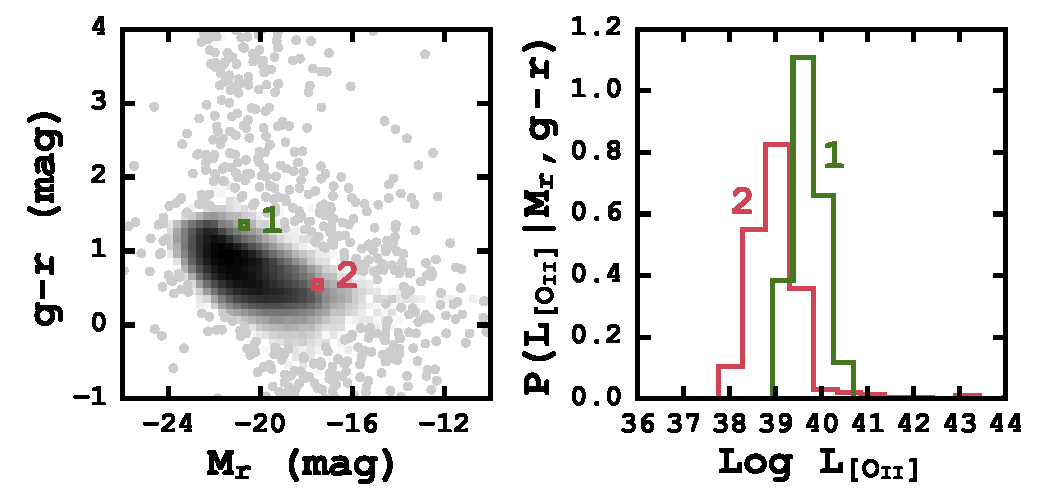
\includegraphics[width=0.9\textwidth]{figures1/oii_sdss.pdf} 
	\caption{\textit{Left}: CMD of 503,113 $z<0.2$ galaxies take from the SDSS DR12 where the shading scales with the density of points. The two colored boxes show regions containing potential catalog galaxies. \textit{Right}: Probability histograms of the Log \hbox{[\ion{O}{ii}]} luminosity for the SDSS galaxies located in the two highlighted regions on the right. The \hbox{[\ion{O}{ii}]} luminosities are assigned to catalog galaxies from slice sampling the probability histogram and converted to fluxes using the redshift of each galaxy.} \label{fig: oii sdss} 
\end{figure*}

This work plans to address these concerns in the following ways. We create and evaluate a HETDEX like selection ``function'' of galaxies over a similarly large portion of the sky and use well adopted techniques to recover the dynamical properties, such as velocity dispersion and cluster mass. In addition to standard techniques of cluster mass estimation, we investigate probability based and machine learning based approaches of cluster mass prediction. We compare these results to a series of targeted galaxy cluster observations, where each member galaxy is assumed to be observed. Each of these observations use realistic uncertainties from galaxy magnitude and line-flux limits. These strategies will better allow future work to predict the number and types of galaxy clusters which should be observed with VIRUS during both the HETDEX survey portion and through targeted follow up observations.

We begin in Section \ref{sec:Data} by giving an overview of what data is used, how it is created, and how we make our ``observations.'' Details about the determination of cluster parameters, velocity dispersion, total mass, etc., are discussed in Section \ref{sec:recovery}. Next, we present the results of our study in Section \ref{sec:results} and discuss their implications in Section \ref{sec:discussion}. Finally we summarize our findings in Section \ref{sec:summary}. A follow-up to this work \citep{Boada2016a} will investigate how the techniques developed here will work in practice. 

Throughout this paper, we adopt the following cosmological model: $\Omega_\Lambda = 0.714$, $\Omega_M = 0.286$, $\sigma_8 = 0.82$ and $H_0= 70$ \kms \mpc (taken from the Buzzard catalogs; see below), assume a Chabrier initial mass function (IMF; \citealt{Chabrier2003}), and use AB magnitudes \citep{Oke1974}.

\section{Data and Mock Observations}\label{sec:Data}
In this section, we describe the data products and the techniques used to replicate the HETDEX survey. We use the information from a large mock galaxy catalog enhanced by the emission line properties of galaxies in the SDSS to create a realistic ``sky'' and ``observe'' it with a HETDEX-like observing strategy.

\subsection{The Buzzard Mock Catalogs}
The Buzzard mock galaxy catalogs cover 398.49 \degsq\ between $4^h< RA < 6^h$ and $-61\degree < DEC < -41\degree$ and are derived from a combination of Sub-halo Abundance Matching (ShAM) and ADDSEDs (Adding Density Dependent Spectral Energy Distributions) tied to an in house n-body cosmological simulation. A brief description of the catalog creation is described as follows. The initial conditions are generated with a second-order Lagrangian perturbation theory using {\sc 2LPTic} \citep{Crocce2006}. Dark matter (DM) n-body simulations are run using {\sc LGadget-2} (a version of {\sc Gadget-2}; \citealt{Springel2005}). The Buzzard catalogs adopt the following cosmological parameters: $\Omega_m = 0.286$, $\Omega_\Lambda = 0.714$, $H_0 = 70$ \kms \mpc, $\sigma_8 = 0.82$, and $n_s = 0.96$. The DM halos are identified using the {\sc ROCKSTAR} halo finder \citep{Behroozi2013} which also calculates halo masses. 

Galaxy $M_r$ luminosities are added to the velocity peaks using ShAM \citep{Reddick2013}, and ADDSEDs assign luminosities in the other bands. A $M_r$-density-SED relation is created using a SDSS training set, and for each mock galaxy the SED of a randomly selected training set galaxy which has a similar $M_r$ and density is assigned. The result is a mock catalog containing 238 million galaxies with $\sdssr < 29$ mag and $z \leq 8.7$.

The catalog information, used in this study, is broken into two large portions. The ``truth'' files contain the characteristics of each individual galaxy, such as right ascension (RA), declination (DEC), redshift ($z$), observed and rest-frame magnitudes, and many others. The ``halo'' files contain information for individual halos, to which many individual galaxies may belong. This includes five estimations of dynamical mass, RA, DEC, z, three dimensional velocity dispersion, and many others. However, the catalogs do not include information for emission lines. We supplement the catalogs by generating this information; the process is described in Section~\ref{sec: oii luminosity}.

% \begin{figure}
% 	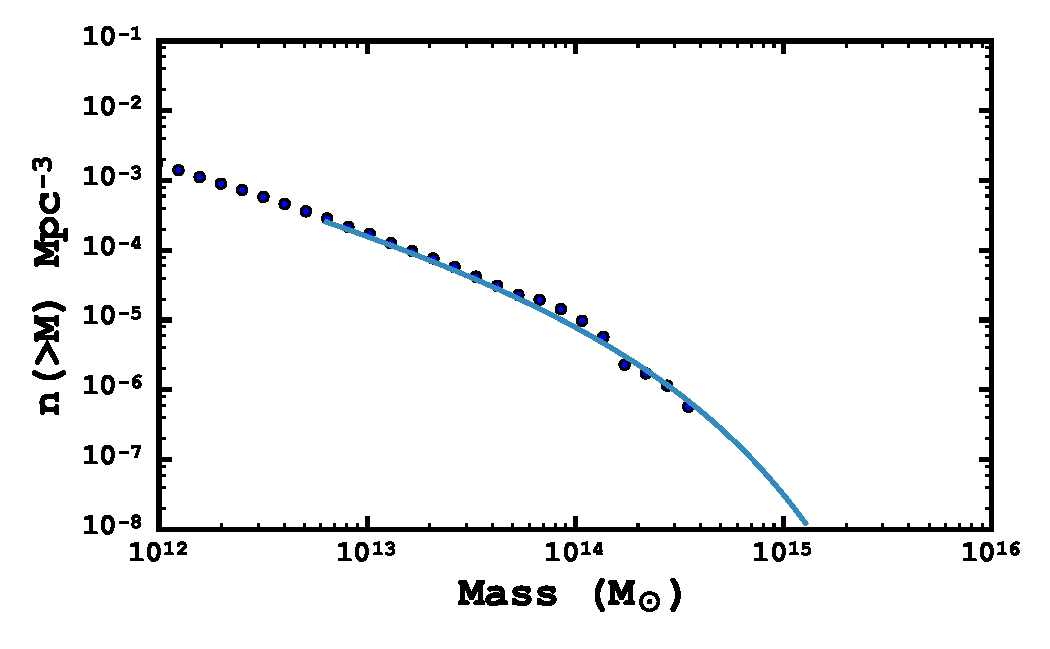
\includegraphics[width=\textwidth]{figures1/hmf.pdf}
% 	\caption{The cumulative MF (from \citealt{Tinker2008}) of halos above $M_{200c}$ at $z=0.1$}
% 	\label{fig: hmf}
% \end{figure}

We investigate the accuracy of the halo mass distribution by comparing the cumulative number density of halos above a mass ($M_{200c}$) threshold to the halo mass function (HMF) of \cite{Tinker2008}. We calculate the HMF at central redshifts of 0.1, 0.2, and 0.4 using {\sc HMFcalc} \citep{Murray2013} and compare it galaxies in a redshift window of $\Delta z\pm0.01$. We find a very good agreement between the predicted HMF and the observed distribution of clusters.

\subsection{Conditional \hbox{[\ion{O}{ii}]} Flux Probability Distribution Functions}\label{sec: oii luminosity}
We use the SDSS DR12 \citep{Alam2015} catalogs to assign \hbox{[\ion{O}{ii}]} emission line strengths to the galaxies in the Buzzard catalog. We use 503,113 objects classified as galaxies selected over $z = 0.02 - 0.2$ with {\sc zwarning $=0$} and a measured \hbox{[\ion{O}{ii}]} line flux signal-to-noise of five. Figure~\ref{fig: oii sdss} shows the color-magnitude diagram (CMD) of $M_r$ and $g-r$ for these galaxies.

To assign an \hbox{[\ion{O}{ii}]} luminosity to each galaxy in our catalog, we place the catalog galaxies on the same CMD and select all SDSS galaxies in a small 2D ($M_r$, $g-r$) bin around the galaxy. We extract all of the SDSS galaxies inside that bin and create a histogram of their \hbox{[\ion{O}{ii}]} luminosities, the right panel of Figure \ref{fig: oii sdss}. Using a slice sampling technique \citep{Neal1997} we assign the catalog galaxy an \hbox{[\ion{O}{ii}]} luminosity based on the distribution of SDSS galaxies in that bin. In very few cases (1.3\% of galaxies) do the $g-r$ and $M_r$ magnitudes of the galaxies in the Buzzard catalog not overlap with the distributions in SDSS. For these objects, we assign them zero \hbox{[\ion{O}{ii}]} flux, but this has no impact on our analysis. For catalog galaxies with have very few ($1\leq N<10$) SDSS galaxies in their respective bin, we assign it the mean \hbox{[\ion{O}{ii}]} flux. 

Figure~\ref{fig: oii sdss} illustrates this process. The numbered boxes in the left panel show the bins corresponding to two example Buzzard galaxies ($M_r, g-r = -17.7,~0.49$ and $M_r, g-r = -21.4,~1.24$). The right panel shows the Log \hbox{[\ion{O}{ii}]} luminosity distribution functions, $P($\hbox{[\ion{O}{ii}]}$| M_r, g-r)$, which we use to assign \hbox{[\ion{O}{ii}]} luminosity to each object. The luminosity is then converted into an \hbox{[\ion{O}{ii}]} flux through 
\begin{equation}
	F = \frac{L}{4\pi D_L}
\end{equation}
where $D_L$ is the luminosity distance \citeeg{Hogg1999}.

\subsection{HETDEX}\label{sec: hetdex}
\begin{figure} 
	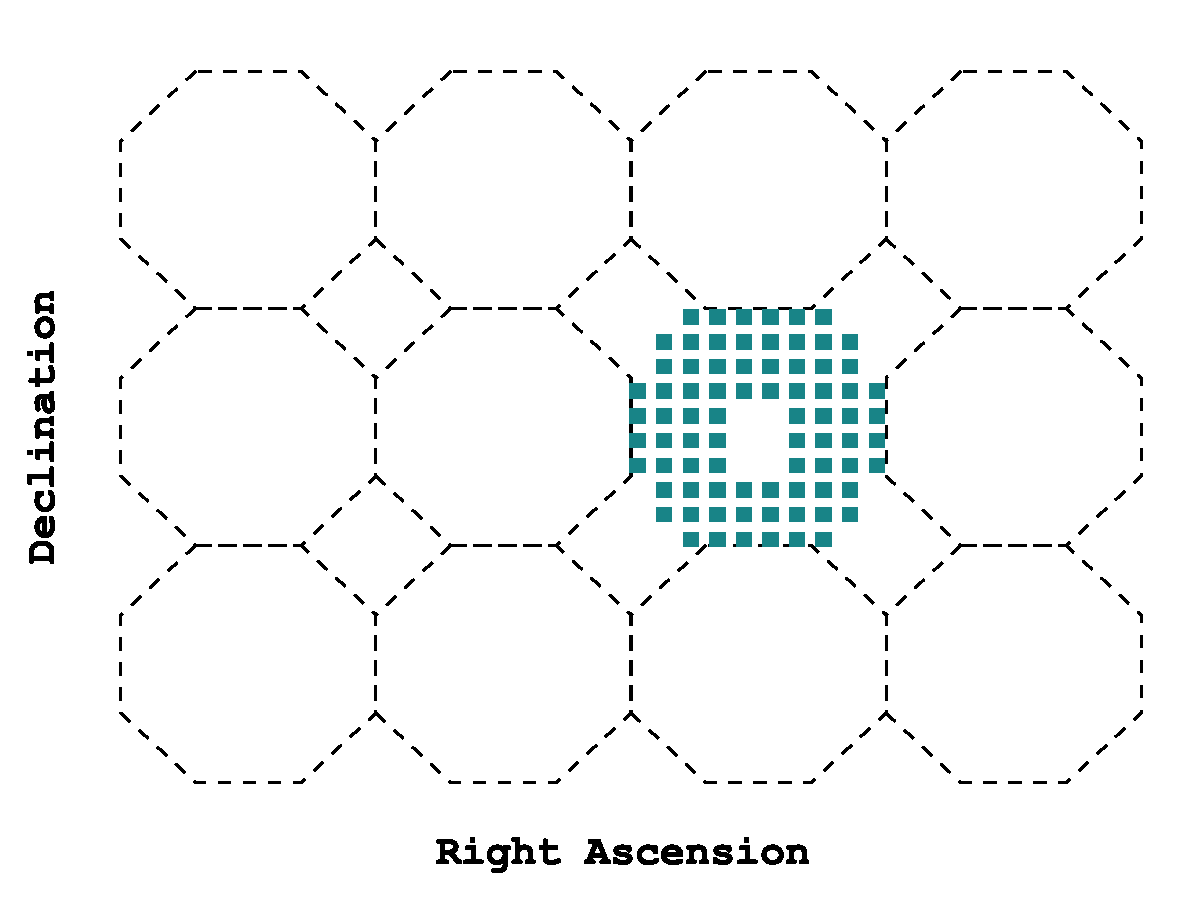
\includegraphics[width=\textwidth]{figures1/pointings.pdf} 
	\caption{Representative observation tiling scheme for the HETDEX $16' \times 16'$ pointings. Each turquoise square represents the position of a single VIRUS IFU, and the dashed octagons approximate the size of a single observation. Inside each IFU HETDEX will achieve near complete coverage through three dithers. See the text for more details.} \label{fig: ifu layout} 
\end{figure}

We designed the results of this study to be used in conjunction with HETDEX, a large, blind, spectroscopic survey. HETDEX will measure the redshifts of $8 \times 10^5$ LAE galaxies between $1.9 < z < 3.5$ using a collection of 78 wide-field IFU spectrographs covering the wavelength region $3500 - 5500$~\AAA\ at R $\sim$ 750 \citep{Hill2008}. The primary science goal of these observations is to provide $<1\%$ accuracy measurements of the Hubble expansion parameter and the angular diameter distance at $z\sim2$. This result will provide significant constraints on the evolution of the dark energy equation of state which is both competitive with, and independent of, constraints derived from observations of the \lya forest.

The entire HETDEX survey will cover 420 \degsq\ with a 1/4.5 filling factor over two fields: a $\sim 300$ \degsq\ northern field, and a $\sim 140$ \degsq\ equatorial region. The spectral coverage allows for the detection of \hbox{[\ion{O}{ii}]} ($\lambda\lambda 3727,3729$) emitters to $z\sim 0.5$ and Ca H ($\lambda 3968.5$) and K ($\lambda 3933.7$) absorption features to $z\sim 0.4$. The $10 \sigma$ detection threshold for spectral features will be $3.5\times10^{-17}$ \ergscm\ at 5000 \AAA, or equivalently, $g = 21.9$ mag for continuum objects. 

The HETDEX IFU pattern is illustrated in Figure~\ref{fig: ifu layout} by the turquoise squares. Each of the 78 IFUs, are comprised of 448 optical fibers subtending a $50'' \times 50''$ region on the sky \citep{Kelz2014}. The inter-IFU spacing is also $50''$, spanning a total area of $16'\times 16'$ on the sky. The individual IFUs have a fill-factor of 1/3, which will be completely filled with three dithers of the telescope at each pointing.

\subsection{Mock Observations}\label{sec: observations}
When selecting galaxies from the Buzzard catalog we assume an observation for all galaxies laying within a turquoise, IFU square in Figure~\ref{fig: ifu layout}. In practice, this is achieved by three dither positions at each pointing. Galaxies which lie between the IFUs are missed, as well as the galaxies which lie between the pointings, as there is no overlap between one pointing and the next. To cover the 398.49 \degsq\ field of the Buzzard catalog we require 5370 pointings where 0.015 \degsq\ of each pointing is covered by an IFU. The total area of the sky covered by an IFU is 80.80 \degsq\ which gives a filling factor of 1/4.65, slightly decreased from the expected filling factor of 1/4.5.

In this work we consider two separate observing strategies, Targeted and Survey. The Targeted observations use ``direct'' observations where each cluster is targeted individually, and every cluster member galaxy is assumed to be observed. The Survey observations mimic the HETDEX observation pattern across the sky, where no cluster is directly targeted and not all cluster member galaxies are observed. Both of these observations have HETDEX-like galaxy detection thresholds (described in the previous subsection), so while a galaxy may be observed, a redshift will only be measured if the galaxy satisfies the continuum brightness or emission line flux limits for the HETDEX survey. For comparison we also include a set of Targeted observations with ``perfect'' knowledge which assume no detection threshold, if a cluster member galaxy is observed, it is also detected. This provides an important best-case scenario, and differs from the true cluster properties between we are still calculating the cluster mass from the observed member galaxy velocity dispersions, and represent the best possible mass estimates using velocity dispersion as the observable. These observations provide three levels of quality with ``Perfect knowledge'' being the highest and Survey being the lowest.

\section{Recovery of Parameters}\label{sec:recovery}
In the following subsections, we outline the methods we use to derive the dynamical properties of the galaxy clusters in our sample. The following is, in many cases, a subset of the available methods to derive any single parameter. The specific choice of method may improve or diminish the accuracy of the recovered parameter, but the methods chosen were to facilitate comparison with other observational studies \citeeg{Kirk2015, Boada2016a}. 

\subsection{Cluster Redshift}
The accurate determination of the cluster redshift ($z_c$) is crucial to the reliability of all following measurements. An incorrect cluster redshift introduces error into the measured line-of-sight velocity (LOSV) and corresponding dispersion, which, in turn, contributes to errors associated with dynamical mass and radius. 

In simple terms, the cluster redshift is the mean of the redshifts of all galaxies associated with the cluster, where the mean is the first moment of the velocity (redshift) distribution function $P(z)$. In practice, the first moment is strongly subject to outliers, so we rely instead on the biweight location estimator \citep{Beers1990} through\footnote{Implemented as part of the {\sc astLib} Python library. See \hbox{http://astlib.sourceforge.net}}:
\begin{equation}
C_{BI} = M + \frac{\sum_{|u_i| < 1} (z_i - M)(1-u_i^2)^2}{\sum_{|u_i| < 1}(1-u_i^2)^2}
\end{equation}
where $z_i$ are the individual redshifts, $M$ is the median redshift and $u_i$ is given by:
\begin{equation}
	u_i = \frac{(z_i - M)}{C\,\mathrm{MAD}}.
\end{equation}
MAD is the median absolute deviation, also defined in \cite{Beers1990}, and $C$ is the a tuning constant. We choose $C=6$ (the suggested value) which balances computational speed and location accuracy. 

Although this work assumes that we know each galaxy's redshift to infinite precision, in practice, we find a simple weighted mean provides a reliable estimate of $z_c$ when there are uncertainties on the individual galaxy redshifts. 

\subsection{Line-of-Sight Velocity Dispersion}\label{sec: LOSVD}
We calculate the LOSV to each galaxy, where
\begin{equation}
	\mathrm{LOSV} = c\frac{z - z_c}{1+z_c}
\end{equation}
and $c$ is the speed of light, $z$ is the redshift of the individual galaxy, and $z_c$ is the overall cluster redshift described in the previous subsection.

We follow the maximum likelihood method of \cite{Walker2006} to estimate the line-of-sight velocity dispersion (LOSVD). We maximize the probability function 
\begin{equation}\label{eq: jointGaussian}
P(\{v_1, ..., v_N\})=\displaystyle\prod_{i=1}^{N}\frac{1}{\sqrt{2\pi(\sigma_i^2+\sigma_{1D}^2)}}\exp\biggl[-\frac{1}{2}\frac{(v_i-\langle u \rangle)^2}{(\sigma_i^2+\sigma_{1D}^2)}\biggr]
\end{equation}
where $\sigma_{1D}$, $\langle\mu\rangle$, and $\sigma_i$ is the LOSVD, the average radial velocity and the error on the individual LOSVs (which we have assumed to be normally distributed) respectively, using a Monte Carlo Markov Chain (MCMC) sampler ({\sc emcee}\footnote{http://dan.iel.fm/emcee/current/}; \citealt{Foreman-Mackey2013}) which is based on affine-invariant ensemble sampler (see \citealt{Goodman2010} for details on affine-invariant samplers). We draw twenty thousand samples from the posterior probability distribution using simple priors, $\langle\mu\rangle$ lies between the maximum and minimum LOSV and $0< \sigma_{1D} < 1400$ \kms. We set the upper limit on the LOSVD as the LOSVD corresponding to a $10^{16}$ \Msol\ cluster at $z\sim0.0$, higher mass than any expected cluster in Buzzard. When the full distribution of LOSVDs is not used, the final LOSVD is quoted as the median value of the posterior probability distribution with 68\% error bars defined as the square root of second moment of the same distribution, the standard deviation.

In principle, a single statistic such as the biweight scale estimator or the gapper estimator (both from \citealt{Beers1990}) with many bootstrap resamplings could be used to construct a distribution of $\sigma_{1D}$. In simple tests where the values of both $\sigma_{1D}$ and $\langle\mu\rangle$ are known, the 68\% error bars derived from the MCMC method give slightly better results with the true LOSVD value bracketed by the error bars in $\sim68\%$ of the cases versus $\sim57\%$ with bootstrapping and a single statistic. In addition, we prefer the maximum likelihood method for its straight forward treatment of the errors in the LOSV measurements, which will become important in the practical application to real data \citeeg{Boada2016a}.

\subsection{Estimates of Cluster Mass}\label{sec: mass}
\subsubsection{Power Law Based Method}
The relationship between the LOSVD and cluster dynamical mass has been the focus of several many \citeeg{Evrard2008, Saro2013, Sifon2013, VanderBurg2014}, where the relationship for the mass enclosed by $r_{200c}$ takes the form
\begin{equation}\label{eq:power law}
	M_{200c} = \frac{10^{15}}{h(z)} \bigg{(}\frac{\sigma_{1D}}{A_{1D}} \bigg{)}^{1/\alpha} \Msol
\end{equation}
with $A_{1D} = 1177 \pm 4.2$ \kms\ (\citealt{Munari2013}; referred to as $\sigma_{15}$ in \citealt{Evrard2008} and other works), $\alpha = 1/3$, $h(z) = H(z)/100$, and $\sigma_{1D}$ is the LOSVD of the velocity tracers (dark matter particles, subhalos or galaxies). $H(z) = H_0 E(z)$ and $E(z) = \sqrt{\Omega_m(1+z^3)+\Omega_{\Lambda}}$.

A growing body of work suggests that there is a significant difference in the observed LOSVD depending on the velocity tracers used. Specifically, while there is little difference between using galaxies and their host DM subhalos, there is a significant over estimation of the LOSVD when using galaxies/subhalos compared to DM particles \citep{Munari2013}. We follow other works \citeeg{Kirk2015, Sifon2015a} using the scaling relation, given in Equation~\ref{eq:power law} to facilitate comparisons with other observational studies, which rely on galaxies as tracers. 

\subsubsection{Other Estimates of Dynamical Mass -- Introduction}
In the following subsections we use two methods to predict the mass of a cluster based on other observables. Often the cluster mass is estimated based on a single observable, X-ray temperature, LOSVD, richness and others (see Section~\ref{sec: Introduction} for referenced examples). Here we combine many observables to attempt to correct the mass inferred solely from the velocity dispersion. The first method is traditional ``probability based'' where we marginalize over a series of observables to find the most probable cluster mass. The second is based on a machine learning (ML) algorithm which attempts to infer the relationship between the observables and the desired output, the cluster mass. Both of these methods are examples of supervised learning algorithms where the relationship between the observable parameters and the target parameter (the cluster mass) are both known.

As with any predictive analysis it is important to test the model on data that the model has not seen before. This prevents over-fitting. In the following subsections we take all of the observed clusters, our full sample, split them, and generate a \emph{training} and \emph{testing} set \citeeg{Ripley2007, Xu2013, Ntampaka2015, Ntampaka2015a, Acquaviva2016}. Traditionally, the training set is a set of data used to infer possibly predictive relationships. The test set of data is then used to assess the correctness of the predictive relationship. Our data is randomly split into 70\% training and 30\% testing. We follow the ML convention and refer to the individual clusters in each set as a ``sample'', and the parameters associated with the cluster ($z$, LOSVD, mass, etc.) as ``features''.

\subsubsection{Probability Based}\label{sec:probability method}
For internal consistency between this and the ML based method we use 70\% of the clusters to establish a conditional probability density of $P(M_{200c} | \vec{x})$ which we then use as the cluster mass probability density for the remaining clusters with similar features. In this way we, ``train'' the probability density using the existing simulated data, and apply it to the ``test'' sample (the remaining 30\% of the data not used as the training set).

\begin{figure*} 
	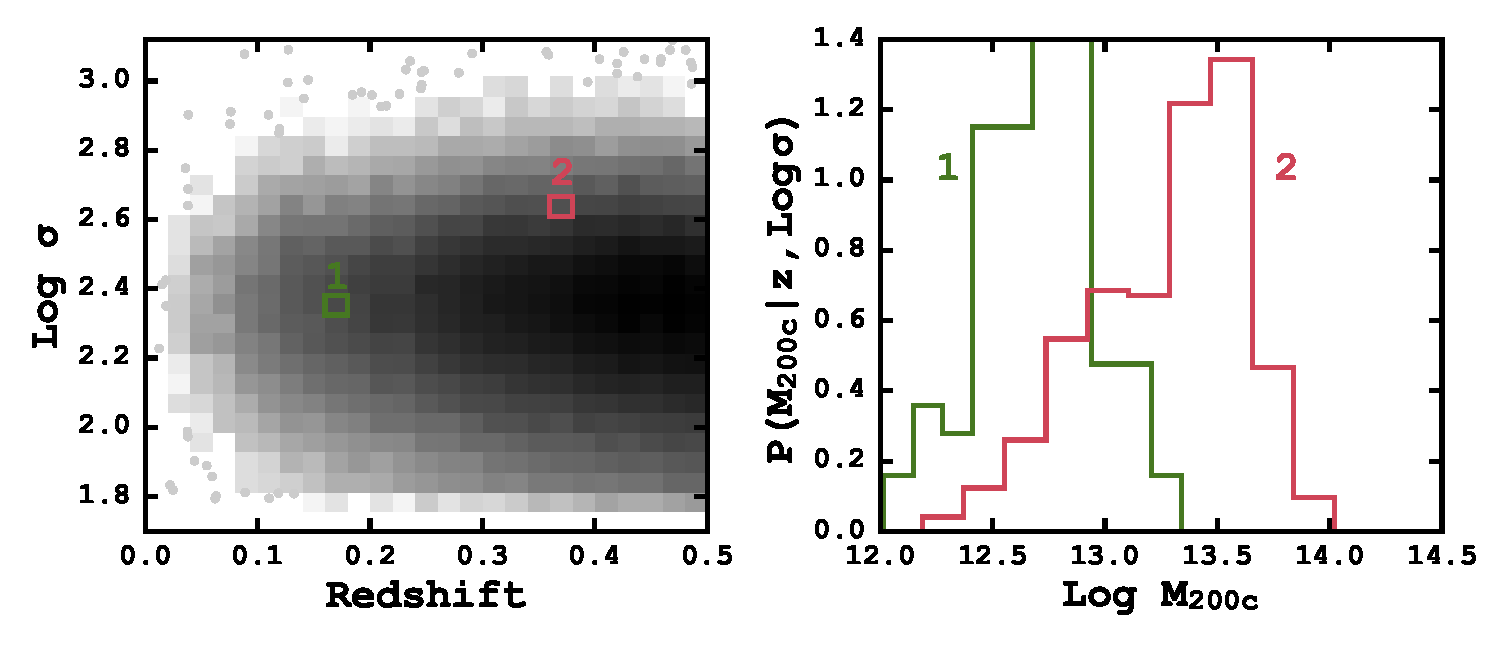
\includegraphics[width=\textwidth]{figures1/prob_example.pdf} 
	\caption{Illustration of the probability based cluster mass prediction method. \emph{Left}: The two dimensional posterior probability distribution of LOSVD and redshift used to determine the correct cluster mass. The pink and green rectangles show the locations of two example galaxies used to create the conditional probability distribution of the mass, $P(M_{200c}|\vec{x})$. \emph{Right}: The conditional probability distribution of the cluster mass for the two example galaxies. See text for a complete description.} \label{fig: probability corner} 
\end{figure*}

In this method, the cluster masses are predicted using the method illustrated in Figure~\ref{fig: probability corner}. The left panel shows the two dimensional (joint probability) projections of the posterior probability distributions of the feature training data. The conditional probability of the cluster mass $P(M_{200c}|\vec{x}= \{ x_1,x_2,...\})$ (shown in the right panel) is determined by selecting a region in the joint probability distribution. For example, using the LOSVD and redshift features we create $P(M_{200c}|\vec{x})$ for two test galaxies, shown by the green and pink boxes in the left panel of Figure~\ref{fig: probability corner}. These example galaxies have features $\vec{x} = \{\sigma=200\, \kms,z=0.16\}$ and $\vec{x} = \{\sigma=400\, \kms,z=0.36\}$. We select all galaxies in our training sample with similar features and create the conditional probability distributions shown in the right panel.

For the clusters making up the \emph{test} sample the mass is unknown (it is what we are trying to predict) but the other features are known. To determine the mass probability distribution of a test cluster, $P(M_{200c})$, we combine the conditional probability distribution, $P(M_{200c}|\vec{x})$, created previously with the probability distribution of $\sigma$, the LOSVD, through Equation~\ref{eq: Pm}.
\begin{equation}\label{eq: Pm}
	P(M_{200c}) = \int P(M_{200c}|\vec{x})\ P(\sigma)\ d\sigma\ P(z)\ dz
\end{equation}
The expected mass is determined by calculating the first moment of the probability density. This becomes our ``predicted'' cluster mass, $M_{pred}$.
\begin{equation}\label{eq: expected mass}
	M_{pred}= \int M_{200c}\ P(M_{200c})\ dM_{200c}
\end{equation}
The confidence interval associated with this prediction can be estimated two ways. First, by calculating the second moment of the probability density through
\begin{equation}\label{eq: variance}
	\mathrm{Var} = \int (M_{200c} - M_{pred})^2\ P(M_{200c})\ dM_{200c}
\end{equation}
or by drawing many samples from $P(M_{200c})$ and calculating the values at the 16th and 84th percentile. In practice we find that both methods produce similar results for a large number of trials. Therefore, we quote predicted masses as the most probable mass given by Equation~\ref{eq: expected mass} and associated 68\% error estimated through the square root of Equation~\ref{eq: variance}.

\subsubsection{Machine Learning Based}\label{sec:machine learning method}
The cluster mass estimation in this section relies on a ML technique known as an ensemble method, where many estimators are created by a single learning method with the goal of improved generalization and robustness compared to a single estimation. Ensemble methods \citeeg{Caruana2006} come in two general flavors. Averaging methods average (hence the name) the estimators to produce a single prediction. Boosting estimators build estimates sequentially by attempting to address poor performing estimators in each previous step, hence ``boosting'' the predictive power.

Here we use an averaging ensemble learning method known as a forest of randomized decision trees, often shorten to just random forest (RF; \citealt{Ho1995, Ho1998}). Decision trees can be visualized a flow chart where forks are the branches of the tree. The path along the tree is decided by the values of the feature(s) at each branch. RF estimators use a random subset of the training set at each fork to decide which path should be followed. The final prediction is then the mean of all the final predictions from the trees. We use RF regression methods as implemented in {\sc Scikit-Learn} \citep{Pedregosa2012}.

The ML method generates ``prediction intervals'' between observed and derived quantities (rather than ``confidence intervals''). A prediction interval is an estimate of the interval encompassing future observations, with a certain probability. And, unlike confidence intervals, which describe uncertainties on the different moments of a population, a prediction interval is unique to each prediction. In many regresson analyses, such as linear fitting, the prediction intervals are based on underlying assumptions of normally distributed residuals. However, RF estimators do not have any such assumptions and require special treatment.

The prediction intervals here are based on the general method of quantile regression forests \citep{Meinshausen2006}. The general idea is that all response variables are recorded, not just the mean. Then the prediction can be returned as the full conditional probability distribution of all responses, which allows us to generate the prediction intervals. We report the 68\% prediction interval as the square root of the second moment of the full conditional probability distribution.

\section{RESULTS}\label{sec:results}
Here we explore the cluster member recovery rate and mass estimates for the two observing strategies, Targeted, and Survey. Targeted observations are direct observations of a cluster where each cluster member galaxy, above the detection thresholds (see Section \ref{sec: observations}), is observed. Survey observations mimic the HETDEX observation strategy such that no cluster is directly observed, and only the cluster member galaxies above the detection threshold and within an IFU (see Figure \ref{fig: ifu layout}) are observed.  We discuss the accuracy of cluster dynamical mass derived from both the power law scaling relation (see Equation \ref{eq:power law}) and through the probability and ML methods. We also compare the results from the Targeted and Survey observing strategies to the results of a ``Perfect'' survey, where the redshift of each galaxy, regardless of observational limits, in the cluster is known perfectly.

\subsection{Recovery of Cluster Members}
\begin{figure*}
	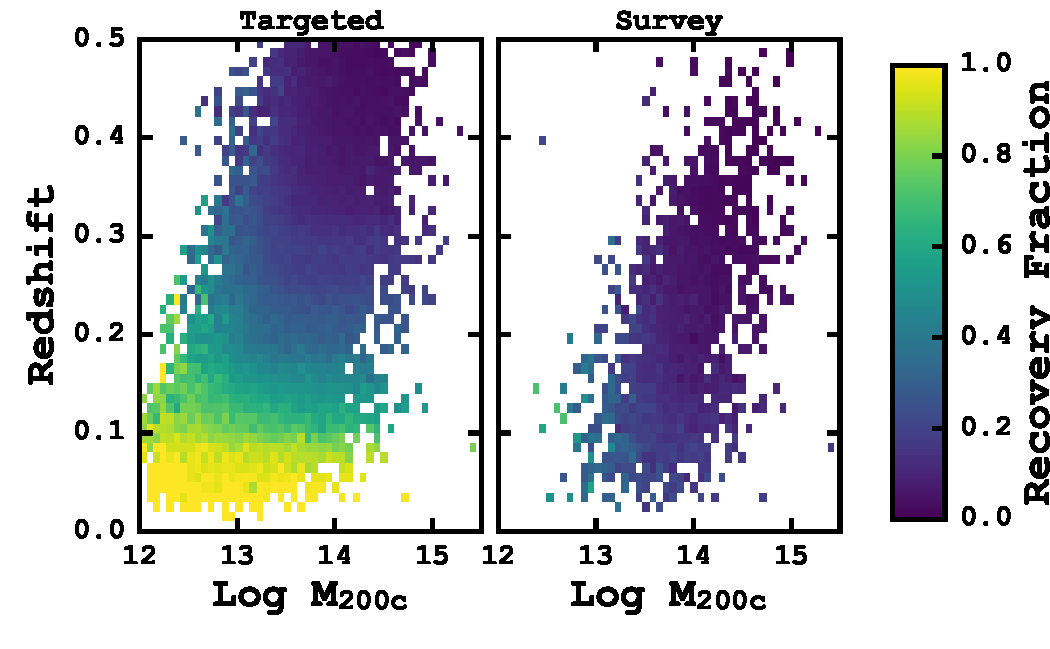
\includegraphics[width=0.8\textwidth]{figures1/recovery.pdf} 
	\caption{Recovery fractions ($N_{obs}/N_{True}$) of cluster member galaxies as a function of redshift and true cluster mass for the Targeted and Survey observing strategies. We have applied HETDEX-like observational limits on the cluster galaxy detection, and require at least five galaxies to be detected for a cluster to be recovered. The shading indicates the mean recovery fraction for clusters within each small bin of redshift and cluster mass. We find a significant decrease in the recovery of galaxies with increasing redshift. This leads to lower recovery fractions of high mass clusters as many only exist at larger redshifts. The significant decline in the number of galaxies observed with the Survey strategy is due to gaps in the VIRUS IFU, where the galaxies are missed.} \label{fig: recovery} 
\end{figure*}

As discussed in Section \ref{sec: observations}, the observational constraints place limits on the total number of clusters member galaxies expected to be recovered. Knowing these limits will provide important information for potential future follow up or Targeted observations. We recover 14,189 clusters with Targeted observations and 1,760 clusters with Survey observations, where we require a detection of $N_{obs} >=5$ galaxies for a cluster to be detected. Figure \ref{fig: recovery} shows the recovery fraction of member galaxies, the number of observed galaxies divided by the number of actual galaxies ($N_{obs}/N_{True}$), as a function of both redshift and cluster mass. As expected, the Targeted observing strategy where the individual clusters are targeted through several dithers to ensure near complete coverage, performs significantly better than the Survey observing strategy across all redshifts and cluster masses. With Perfect knowledge, recovery fraction would be unity across all redshifts and cluster masses where clusters exist.

For the Targeted observations, shown in the left panel of Figure~\ref{fig: recovery}, the pattern of decreasing recovery fraction as a function of redshift (y-direction) is due to the observational limits imposed. Because HETDEX is limited in apparent magnitude, we expect to recover fewer galaxies at higher redshift, where the galaxies are often below our $5\sigma$ detection threshold. For example, we tested this by constructing an artificial HETDEX-like survey, limited by volume for all galaxies with $M_g < -11$. In this case, our recovery fraction increases to $>70$\%, which shows that the flux limit is dominating the (lower) recovery of our flux-limited survey.

For the recovery fraction as a function of true cluster mass (x-direction), we find a general decrease in the recovery fraction of member galaxies with increasing cluster mass. This  is entirely a result of the flux limited survey (see previous paragraph). Because there are few high mass ($M_{200c}>5\times10^{14}$ \Msol) clusters, many of which are at moderately high redshift, the higher redshift cluster members suffer from the limiting apparent magnitude and suppress the recovery fraction at fixed mass. If we were to limit the Survey to $z<0.2$ we find the recovery fraction of clusters, across all masses, increases substantially, and we find a much more consistent detection fraction across all masses. 

For the Survey observations, the right panel of Figure~\ref{fig: recovery}, all of the same effects are at work. In addition we find that the fill factor, due to the gaps between the VIRUS IFUs, further reduces the number of cluster members detected. The median recovery fraction in Survey observations is almost exactly 4.5 times less than the Targeted median recovery fraction. As the total filling factor of the Survey observations increases the two lines will converge.

The recovery fractions in Figure~\ref{fig: recovery} are an outcome of the magnitude limit and \hbox{[\ion{O}{ii}]} line-flux limit of the survey. For Perfect observations, we would detect all members across all cluster masses and redshifts. Recovery fractions of clusters located a the low end of the redshift distribution will improve the most by follow-up targeted observations. But generally, the number of members observed (and subsequently more accurate cluster mass estimates) will benefit from follow-up observations regardless of the redshift. So follow-up observations should be tailored to the specific science goal.

\subsection{Mass estimates}
\begin{figure*} 
	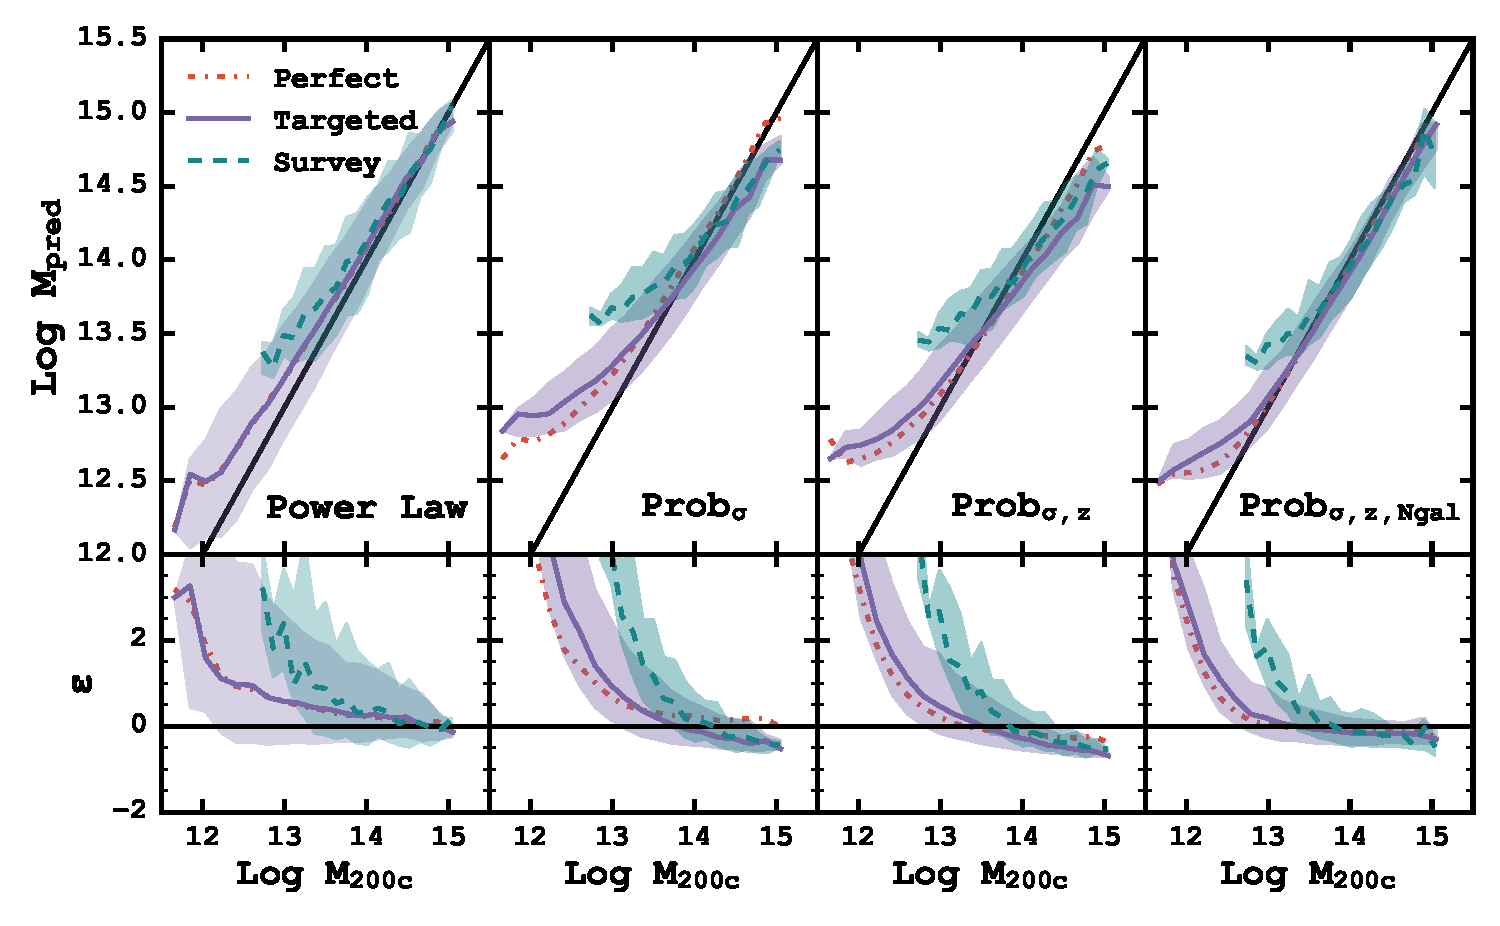
\includegraphics[width=\textwidth]{figures1/Probcomparison.pdf} 
	\caption{Mass predictions for the power law scaling relation (Equation~\ref{eq:power law}) and the probability based technique with different input features as a function of true cluster mass. The bottom row of panels shows the fractional error (Equation~\ref{eq: fractional error}) also as a function of true cluster mass. The solid black line shows the 1:1 relation, in both panels, between $M_{200c}$ and $M_{pred}$. The orange, dash-dotted line is the median predicted mass for perfect observations. The solid, purple line is the median predicted mass for the Targeted observing, and the green, dashed line is the median recovered mass for the HETDEX-like observations. The shaded regions represent the 68\% scatter around the median values.} \label{fig:Probability comparison} 
\end{figure*}

In this section we discuss the accuracy of the recovered masses compared to the true cluster mass from a set of observations. We report on three methods, the power law based approach (Eq. \ref{eq:power law}), the probability based approach (Section \ref{sec:probability method}) and the ML based method (Section \ref{sec:machine learning method}). For each method we consider observations with Perfect knowledge, Targeted observations and Survey observations. The cluster masses presented here are recovered using the best possible conditions, where we have perfect knowledge of the cluster membership. In reality, the mass recovery levels presented in this section represent an upper bound (the best) on the accuracy achievable through this method.

Because it represents the best possible scenario, the Perfect knowledge observations should serve as a baseline to compare the power law based, probability based and ML cluster mass recovery methods. And, while there are many possible metrics to evaluate performance, we compute two: the average bias (given in Table \ref{tbl:mass bias})
\begin{equation}\label{eqn: bias}
\mathrm{\mu_{bias}}(y,y_{pred}) = \frac{1}{N} \sum_{i=1}^N (y_{pred,i} - y_i).
\end{equation}
where $y$ are the true values and $y_{pred}$ are the predicted values, and the scatter about the bias (given in Table \ref{tbl:mass scatter})
\begin{equation}\label{eqn: scatter}
	\sigma_{bias}(y,y_{pred}, \mu_{bias}) = \bigg{[}\frac{1}{N-1} \sum_{i=1}^N (y_{pred,i} - y_i - \mu_{bias})^2 \bigg{]}^{1/2}
\end{equation}
with $N$ clusters in a given bin. Both metrics evaluate how closely the ensemble of predicted cluster masses are to the true cluster masses.

We begin with the Perfect knowledge observations. These observations are of the same clusters as the Targeted observations but without any observational limits. The cluster masses predicted by Equation \ref{eq:power law} gives the following results. For clusters with masses between Log M/\Msol $= 13 - 15.5$, we find $\mu_{bias} = 0.148\pm{0.008}$ dex and $\sigma_{bias} = 0.193\pm{0.001}$. The scatter in recovered masses can be attributed to both physical and numerical effects. The presence of any in-falling matter onto lower mass clusters can introduce a significant amount of substructure, leading to artificial biasing of the measured LOSVD to higher values, increasing the predicted mass \citeeg{Ntampaka2015}. Also, as the number of cluster galaxies decreases the LOSVD PDF is poorly sampled leading to poorly recovered cluster masses due to numerical effects. 

For the Targeted and Survey observations the power law predicted cluster masses give $\mu_{bias} =0.135\pm{0.003}$ dex, $\sigma_{bias} = 0.370\pm{0.002}$ and $\mu_{bias} =0.148\pm{0.008}$ dex, $\sigma_{bias} = 0.324\pm{0.006}$ , respectively. So for the clusters that we detect with Survey observations, we obtain similar levels of accuracy as to the Targeted observations, on the average. This does not mean that the Survey observations cannot be improved by Targeted observations. In fact, when comparing only the galaxies which overlap between the two samples the bias and scatter of the Targeted observations is significantly decreased as more cluster member galaxies are detected, better sampling the LOSVD PDF. The Targeted observations performs similarly on the average because many lower mass clusters are included in the sample, increasing the bias of the overall sample.

\begin{figure*} 
	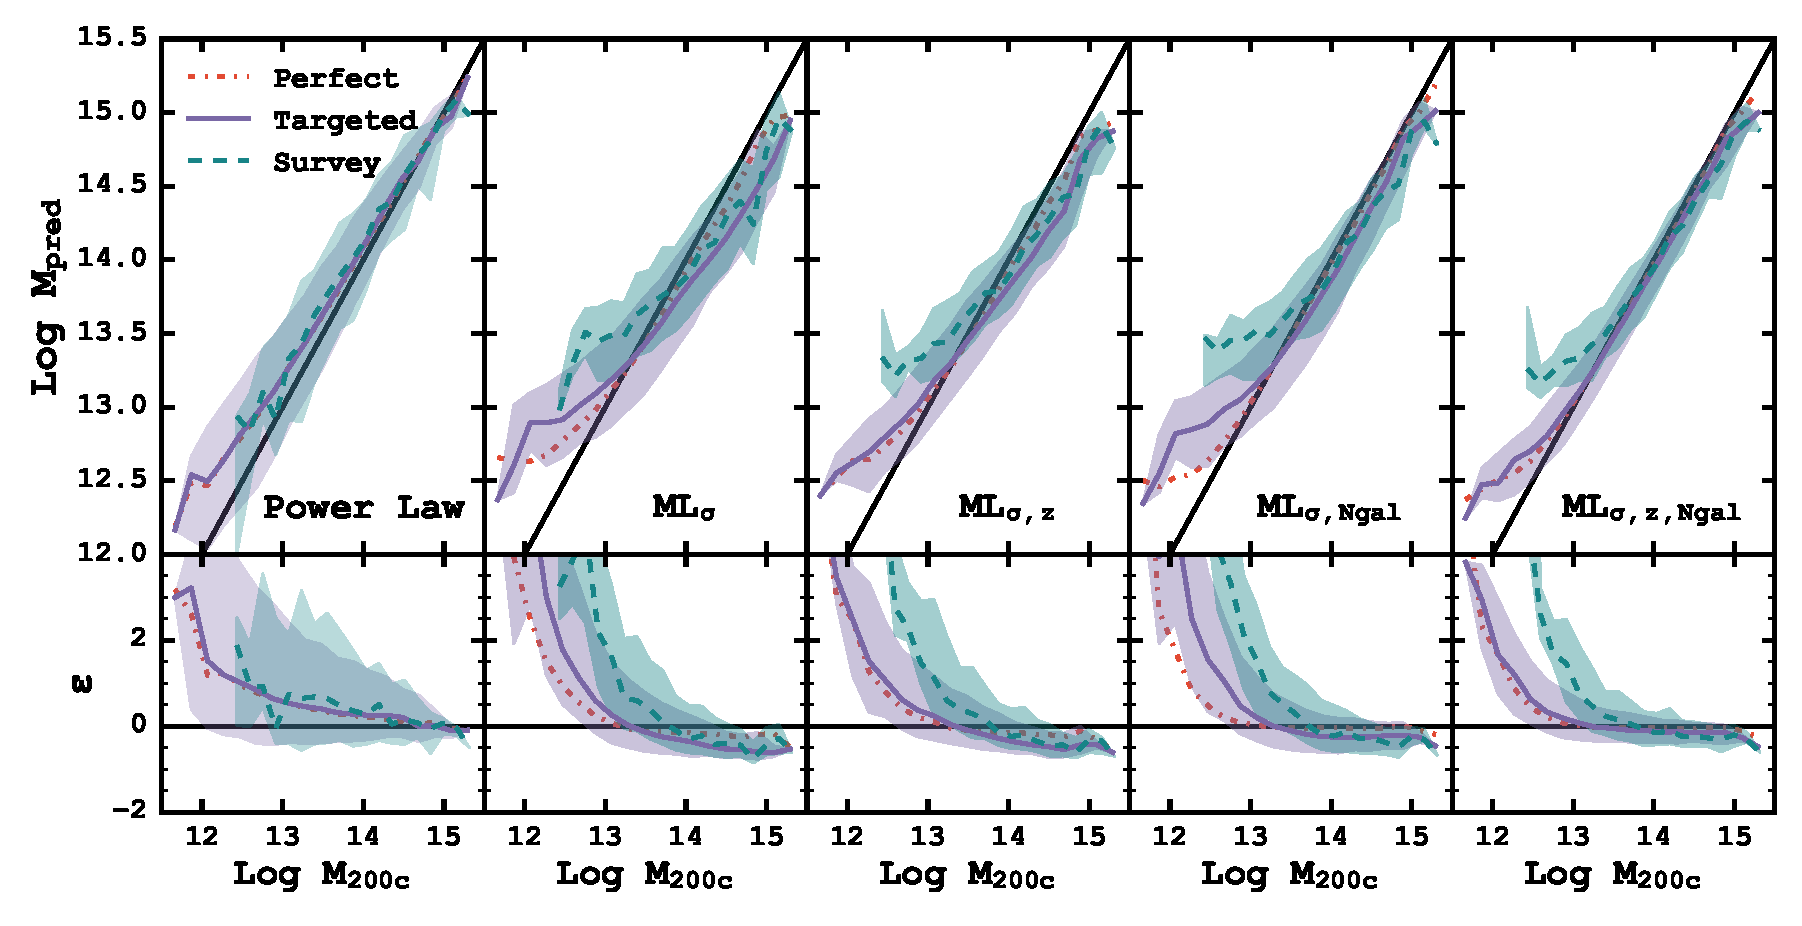
\includegraphics[width=\textwidth]{figures1/MLcomparison.pdf} 
	\caption{Mass predictions for the power law scaling relation (Equation~\ref{eq:power law}) and the ML based technique with different input features as a function of true cluster mass. The bottom row of panels shows the fractional error (Equation~\ref{eq: fractional error}) also as a function of true cluster mass. The solid black line shows the 1:1 relation. The orange, dash-dotted line is the median predicted mass for perfect observations. The solid, purple line is the median predicted mass for the Targeted observing, and the green, dashed line is the median recovered mass for the HETDEX-like observations. The shaded regions represent the 68\% scatter around the median values.} \label{fig: ML comparison} 
\end{figure*}

In both Figures \ref{fig:Probability comparison} and \ref{fig: ML comparison}, we show the predicted ($M_{pred}$) versus true ($M_{200c}$) cluster masses for each of the two observing strategries. The lower panels show the fractional cluster mass error defined as: 
\begin{equation}\label{eq: fractional error}
	\epsilon = (M_{pred} - M_{200c})/M_{200c}
\end{equation}
where $M_{pred}$ is the predicted cluster mass and $M_{200c}$ is the true cluster mass. Higher values of $\epsilon$ indicate the predicted cluster mass exceeds the true cluster mass.

Qualitatively, the top panels of Figures \ref{fig:Probability comparison} and \ref{fig: ML comparison} show that both the probability based and ML based methods out perform (closer to the black 1:1 relation) the power law method when taking advantage of other cluster observables ($z$, $N_{gal}$, etc.). Generally, we find that the single parameter probability and ML methods perform significantly poorer than the power law method, especially at low cluster masses. When combined with the cluster redshift, the predicted cluster masses are improved, because the range of cluster masses decrease with increasing redshift (see Figure~\ref{fig: recovery}). The final addition of the number of observed galaxies, $N_{gal}$ acts as a type of richness estimate, and significantly improves both the bias and the amount of scatter in the predicted masses.

\begin{landscape}
\begin{table}
\centering
\small
\caption{Mean bias (Eqn.~\ref{eqn: bias}) for different bins of predicted cluster mass. This table shows the bias in the predicted cluster mass for the perfect (top section), Targeted (middle section), and Survey (bottom section) observations in different predicted mass bins. The different mass recovery strategies are given in the leftmost column. It can be used to understand how the predicted cluster mass differs from the true cluster masses. Positive numbers indicate the predicted cluster mass over estimates when compared to the true cluster mass.}
\begin{tabular}{cccccccc} 
		&& \multic{6}{Bins -- Log $M_{pred}$} \\
		\cline{3-8} 
		\multicolumn{2}{c}{Method} & $12.5-13$ & $13-13.5$ & $13.5-14$ & $14-14.5$ & $14.5-15$ & $15-15.5$ \\
		\hline
		&& \multic{6}{Perfect Observations} \\
		\hline
		\multicolumn{2}{c}{Power Law} & $0.23\pm{0.007}$ & $0.16\pm{0.003}$ & $0.11\pm{0.002}$ & $0.07\pm{0.004}$ & $0.02\pm{0.011}$ & $-0.07\pm{0.045}$ \\
		\hline 
		\rottext{3}{Prob} &$\sigma$ & $0.32\pm{0.005}$ & $0.16\pm{0.003}$ & $0.10\pm{0.002}$ & $0.07\pm{0.004}$ & $0.05\pm{0.012}$ & $-0.18\pm{0.078}$ \\
		&$\sigma, z$ & $0.17\pm{0.005}$ & $0.01\pm{0.003}$ & $-0.06\pm{0.002}$ & $-0.11\pm{0.015}$ & $-0.14\pm{0.012}$ & $-0.38\pm{0.159}$ \\
		&$\sigma, z, N_{gal}$ & $0.04\pm{0.009}$ & $-0.02\pm{0.002}$ & $-0.02\pm{0.002}$ & $-0.05\pm{0.014}$ & $-0.22\pm{0.126}$ & \nd \\
		\hline
		\rottext{4}{ML} &$\sigma$ & $0.14\pm{0.006}$ & $-0.01\pm{0.003}$ & $-0.07\pm{0.003}$ & $-0.09\pm{0.005}$ & $-0.11\pm{0.014}$ & $-0.17\pm{0.090}$ \\
		&$\sigma, z$ & $0.12\pm{0.005}$ & $-0.01\pm{0.003}$ & $-0.06\pm{0.003}$ & $-0.08\pm{0.004}$ & $-0.11\pm{0.012}$ & $-0.24\pm{0.076}$ \\
		&$\sigma, N_{gal}$ & $0.04\pm{0.004}$ & $-0.02\pm{0.002}$ & $-0.02\pm{0.002}$ & $-0.02\pm{0.002}$ & $-0.02\pm{0.006}$ & $-0.08\pm{0.041}$ \\
		&$\sigma, z, N_{gal}$ & $0.04\pm{0.003}$ & $-0.02\pm{0.002}$ & $-0.02\pm{0.001}$ & $-0.02\pm{0.002}$ & $-0.02\pm{0.005}$ & $-0.08\pm{0.043}$ \\
		\hline
		
		&& \multic{6}{Targeted Observations} \\
		\hline
		\multicolumn{2}{c}{Power Law} & $0.20\pm{0.008}$ & $0.13\pm{0.005}$ & $0.10\pm{0.005}$ & $0.09\pm{0.007}$ & $0.02\pm{0.014}$ & $-0.08\pm{0.043}$ \\
		\hline
		\rottext{3}{Prob} &$\sigma$ & $0.40\pm{0.005}$ & $0.17\pm{0.003}$ & $0.02\pm{0.004}$ & $-0.08\pm{0.006}$ & $-0.19\pm{0.015}$ & $-0.35\pm{0.122}$ \\
		&$\sigma, z$ & $0.25\pm{0.005}$ & $0.08\pm{0.003}$ & $-0.06\pm{0.003}$ & $-0.21\pm{0.015}$ & $-0.35\pm{0.016}$ & $-0.59\pm{0.145}$ \\
		&$\sigma, z, N_{gal}$ & $0.13\pm{0.004}$ & $0.01\pm{0.003}$ & $-0.05\pm{0.003}$ & $-0.12\pm{0.018}$ & $-0.44\pm{0.177}$ & \nd \\
		\hline
		\rottext{4}{ML} &$\sigma$ & $0.26\pm{0.006}$ & $0.02\pm{0.004}$ & $-0.13\pm{0.005}$ & $-0.24\pm{0.008}$ & $-0.35\pm{0.022}$ & $-0.39\pm{0.054}$ \\
		&$\sigma, z$ & $0.18\pm{0.005}$ & $0.03\pm{0.003}$ & $-0.10\pm{0.004}$ & $-0.21\pm{0.006}$ & $-0.31\pm{0.021}$ & $-0.33\pm{0.063}$ \\
		&$\sigma, N_{gal}$ & $0.22\pm{0.005}$ & $0.00\pm{0.004}$ & $-0.13\pm{0.004}$ & $-0.16\pm{0.007}$ & $-0.13\pm{0.014}$ & $-0.19\pm{0.059}$ \\
		&$\sigma, z, N_{gal}$ & $0.09\pm{0.004}$ & $-0.01\pm{0.002}$ & $-0.05\pm{0.002}$ & $-0.08\pm{0.004}$ & $-0.08\pm{0.010}$ & $-0.19\pm{0.060}$ \\
		\hline
		
		&& \multic{6}{Survey Observations} \\
		\hline
		\multicolumn{2}{c}{Power Law} & $0.17\pm{0.068}$ & $0.17\pm{0.023}$ & $0.13\pm{0.014}$ & $0.07\pm{0.014}$ & $0.01\pm{0.022}$ & $-0.09\pm{0.062}$ \\
		\hline
		\rottext{3}{Prob} & $\sigma$ & $0.77\pm{0.030}$ & $0.42\pm{0.011}$ & $0.18\pm{0.008}$ & $-0.03\pm{0.009}$ & $-0.18\pm{0.017}$ & $-0.39\pm{0.102}$ \\
		&$\sigma, z$ & $0.61\pm{0.036}$ & $0.29\pm{0.012}$ & $0.08\pm{0.008}$ & $-0.11\pm{0.009}$ & $-0.38\pm{0.118}$ & $-0.48\pm{0.127}$ \\
		&$\sigma, z, N_{gal}$ & $0.48\pm{0.038}$ & $0.18\pm{0.011}$ & $0.02\pm{0.007}$ & $-0.08\pm{0.008}$ & $-0.50\pm{0.203}$ & \nd \\
		\hline
		\rottext{4}{ML} &$\sigma$ & $0.57\pm{0.046}$ & $0.24\pm{0.015}$ & $0.02\pm{0.012}$ & $-0.17\pm{0.013}$ & $-0.28\pm{0.027}$ & $-0.27\pm{0.117}$ \\
		&$\sigma, z$ & $0.48\pm{0.034}$ & $0.20\pm{0.013}$ & $0.03\pm{0.009}$ & $-0.13\pm{0.011}$ & $-0.26\pm{0.021}$ & $-0.31\pm{0.110}$ \\
		&$\sigma, N_{gal}$ & $0.55\pm{0.043}$ & $0.22\pm{0.013}$ & $0.00\pm{0.010}$ & $-0.14\pm{0.011}$ & $-0.22\pm{0.025}$ & $-0.19\pm{0.079}$ \\
		&$\sigma, z, N_{gal}$ & $0.42\pm{0.029}$ & $0.13\pm{0.011}$ & $-0.00\pm{0.007}$ & $-0.08\pm{0.008}$ & $-0.14\pm{0.016}$ & $-0.19\pm{0.079}$ \\
	\hline
	\end{tabular}
\label{tbl:mass bias}
\end{table}
\end{landscape}

We quantify the bias and scatter for all of the different cluster mass recovery strategies and observing methods in Table \ref{tbl:mass bias} and Table \ref{tbl:mass scatter}. It serves as a type of look up table for future cluster observations with HETDEX. The columns represent bins of predicted galaxy cluster mass and the individual values show the bias and scatter of the true cluster mass. The three horizontal sections represent Perfect, Targeted and Survey observations respectively. So, for example, if a cluster mass is predicted using the $\mathrm{ML}_{\sigma, z}$ method and Targeted observations to be Log M/\Msol\ $=13-13.5$, it is biased upward by $0.03\pm{0.003}$ dex and has a scatter of $0.24\pm0.009$ dex. 

\begin{table*}
\centering
\caption{Scatter (Eqn.~\ref{eqn: scatter}) in cluster mass after bias correction for different bins of predicted cluster mass. This table shows the scatter in the predicted cluster mass for the perfect (top section), Targeted (middle section), and Survey (bottom section) observations in different predicted mass bins. The different mass recovery strategies are given in the leftmost column. It can be used to understand how the predicted cluster mass differs from the true cluster masses.}
\begin{tabular}{cccccccc} 
		&& \multic{6}{Bins -- Log $M_{pred}$} \\
		\cline{3-8} 
		\multicolumn{2}{c}{Method} & $12.5-13$ & $13-13.5$ & $13.5-14$ & $14-14.5$ & $14.5-15$ & $15-15.5$ \\
		\hline 
		&& \multic{6}{Perfect Observations} \\
		\hline
		\multicolumn{2}{c}{Power Law} & $0.34\pm{0.005}$ & $0.22\pm{0.002}$ & $0.16\pm{0.002}$ & $0.14\pm{0.003}$ & $0.14\pm{0.008}$ & $0.11\pm{0.040}$ \\
		\hline 
		\rottext{3}{Prob} &$\sigma$ & $0.26\pm{0.004}$ & $0.20\pm{0.002}$ & $0.16\pm{0.002}$ & $0.14\pm{0.003}$ & $0.16\pm{0.009}$ & $0.19\pm{0.071}$ \\
		&$\sigma, z$ & $0.23\pm{0.003}$ & $0.19\pm{0.002}$ & $0.16\pm{0.002}$ & $0.55\pm{0.010}$ & $0.16\pm{0.009}$ & $0.39\pm{0.143}$ \\
		&$\sigma, z, N_{gal}$ & $0.47\pm{0.007}$ & $0.14\pm{0.001}$ & $0.10\pm{0.001}$ & $0.54\pm{0.010}$ & \nd & \nd \\
		\hline
		\rottext{4}{ML}	&$\sigma$ & $0.29\pm{0.004}$ & $0.24\pm{0.002}$ & $0.21\pm{0.002}$ & $0.19\pm{0.004}$ & $0.18\pm{0.010}$ & $0.22\pm{0.081}$ \\
		&$\sigma, z$ & $0.24\pm{0.003}$ & $0.20\pm{0.002}$ & $0.18\pm{0.002}$ & $0.16\pm{0.003}$ & $0.16\pm{0.009}$ & $0.19\pm{0.068}$ \\
		&$\sigma, N_{gal}$ & $0.19\pm{0.003}$ & $0.14\pm{0.001}$ & $0.10\pm{0.001}$ & $0.08\pm{0.002}$ & $0.07\pm{0.004}$ & $0.10\pm{0.037}$ \\
		&$\sigma, z, N_{gal}$ & $0.17\pm{0.002}$ & $0.13\pm{0.001}$ & $0.10\pm{0.001}$ & $0.07\pm{0.001}$ & $0.07\pm{0.004}$ & $0.11\pm{0.039}$ \\
		\hline
		
		&& \multic{6}{Targeted Observations} \\
		\hline
		 \multicolumn{2}{c}{Power Law} & $0.43\pm{0.006}$ & $0.39\pm{0.004}$ & $0.33\pm{0.004}$ & $0.27\pm{0.005}$ & $0.18\pm{0.010}$ & $0.11\pm{0.039}$ \\
		 \hline
		\rottext{3}{Prob} &$\sigma$ & $0.24\pm{0.003}$ & $0.25\pm{0.002}$ & $0.25\pm{0.003}$ & $0.22\pm{0.004}$ & $0.19\pm{0.011}$ & $0.30\pm{0.110}$ \\
		&$\sigma, z$ & $0.24\pm{0.003}$ & $0.24\pm{0.002}$ & $0.23\pm{0.002}$ & $0.56\pm{0.011}$ & $0.21\pm{0.012}$ & $0.36\pm{0.131}$ \\
		&$\sigma, z, N_{gal}$ & $0.20\pm{0.003}$ & $0.19\pm{0.002}$ & $0.17\pm{0.002}$ & $0.67\pm{0.013}$ & \nd & \nd \\
		\hline
		\rottext{4}{ML} &$\sigma$ & $0.30\pm{0.004}$ & $0.32\pm{0.003}$ & $0.32\pm{0.003}$ & $0.30\pm{0.006}$ & $0.29\pm{0.016}$ & $0.13\pm{0.049}$ \\
		&$\sigma, z$ & $0.26\pm{0.004}$ & $0.25\pm{0.002}$ & $0.24\pm{0.003}$ & $0.23\pm{0.004}$ & $0.27\pm{0.015}$ & $0.16\pm{0.057}$ \\
		&$\sigma, N_{gal}$ & $0.27\pm{0.004}$ & $0.27\pm{0.003}$ & $0.27\pm{0.003}$ & $0.25\pm{0.005}$ & $0.18\pm{0.010}$ & $0.15\pm{0.053}$ \\
		&$\sigma, z, N_{gal}$ & $0.21\pm{0.003}$ & $0.18\pm{0.002}$ & $0.16\pm{0.002}$ & $0.14\pm{0.003}$ & $0.12\pm{0.007}$ & $0.15\pm{0.054}$ \\
		\hline
		
		&& \multic{6}{Survey Observations} \\
		\hline
		\multicolumn{2}{c}{Power Law} &$0.40\pm{0.050}$ & $0.41\pm{0.016}$ & $0.38\pm{0.010}$ & $0.32\pm{0.010}$ & $0.25\pm{0.016}$ & $0.15\pm{0.056}$ \\
		\hline
		\rottext{3}{Prob} &$\sigma$ & $0.11\pm{0.024}$ & $0.18\pm{0.008}$ & $0.22\pm{0.006}$ & $0.22\pm{0.007}$ & $0.19\pm{0.012}$ & $0.25\pm{0.092}$ \\
		&$\sigma, z$ & $0.13\pm{0.028}$ & $0.19\pm{0.008}$ & $0.22\pm{0.006}$ & $0.21\pm{0.007}$ & $1.31\pm{0.084}$ & $0.32\pm{0.115}$ \\
		&$\sigma, z, N_{gal}$ & $0.14\pm{0.030}$ & $0.18\pm{0.008}$ & $0.19\pm{0.005}$ & $0.19\pm{0.006}$ & \nd & \nd \\
		\hline
		\rottext{4}{ML} &$\sigma$ & $0.27\pm{0.034}$ & $0.27\pm{0.011}$ & $0.31\pm{0.008}$ & $0.30\pm{0.009}$ & $0.30\pm{0.019}$ & $0.29\pm{0.106}$ \\
		&$\sigma, z$ & $0.20\pm{0.025}$ & $0.24\pm{0.009}$ & $0.24\pm{0.006}$ & $0.25\pm{0.008}$ & $0.24\pm{0.015}$ & $0.27\pm{0.100}$ \\
		&$\sigma, N_{gal}$ & $0.25\pm{0.032}$ & $0.23\pm{0.009}$ & $0.27\pm{0.007}$ & $0.26\pm{0.008}$ & $0.27\pm{0.018}$ & $0.20\pm{0.072}$ \\
		&$\sigma, z, N_{gal}$ & $0.17\pm{0.021}$ & $0.21\pm{0.008}$ & $0.20\pm{0.005}$ & $0.19\pm{0.006}$ & $0.17\pm{0.011}$ & $0.20\pm{0.071}$ \\
		 \hline
	\end{tabular}
\label{tbl:mass scatter}
\end{table*}

A few caveats apply to the numbers given in Table \ref{tbl:mass bias} and Table \ref{tbl:mass scatter}. While we provide corrections for cluster masses above $10^{15}$ \msol, they are estimated from only a handful of objects, and do not constitute a representative sample of clusters. This becomes particularly apparent for the probability methods with many features. As the number of observed features increases, the number of training clusters in any particular bin decreases. This leads to highly skewed biases and scatters for the high mass clusters and probability methods. We do not report any bin where such small number statistics dominate in Tables~\ref{tbl:mass bias} and \ref{tbl:mass scatter}. On the opposite end of the cluster mass spectrum, there are very few, if any, clusters detected with Targeted or Survey observations below $5\times10^{12}$ \msol. Therefore, while we show these points in Figures~\ref{fig:Probability comparison} and \ref{fig: ML comparison}, we exclude their biases and scatters from Tables~\ref{tbl:mass bias} and \ref{tbl:mass scatter} for the same reasons. 
 
The method which produce the lowest scatter and bias depends on the mass of the cluster in question and the type of observations used. For the Targeted observations, the power law method outperforms all other methods, in terms of bias and scatter, for the highest mass clusters. But outside of the two highest mass bins, the $\mathrm{ML}_{\sigma, z, N_{gal}}$ method shows the smallest amount of scatter and bias most consistently. With Survey observations, the power law again provides the lowest bias in the highest cluster mass bins, but is outperformed in terms of scatter by the other two methods. The $\mathrm{ML}_{\sigma, z, N_{gal}}$ method shows the smallest amount of scatter and bias most consistently across the cluster mass range in question.
 
\subsection{Impact of Training Sample Cosmology}
All simulations (including that used for Buzzard) use specific values for cosmological parameters. When using simulation data to train ML methods, we incorporate all of those assumptions into the learned feature associations. One could imagine that the specific values of the cosmological parameters in the training sample could bias the ML results when applied to data (real or simulated) created from an unknown true set of cosmological parameters. 

To test for this, we used the Millennium simulation as an alternative data set. The Millennium simulation uses a set of cosmological parameters that are substantially different from Buzzard. The Millennium simulation adopts a flat cosmological model based of the values derived from the Two-degree Field Galaxy Redshift Survey \citep{Colless2001} and the first year data of the \emph{Wilkinson Microwave Anisotropy Probe} (WMAP; \citealt{Spergel2003}): $\Omega_\Lambda = 0.75$, $\Omega_M = 0.25$, $\sigma_8 = 0.9$, $n_s = 1$ and $H_0= 73$ \kms \mpc. The clusters in Millennium provide a testing sample to understand how a training sample derived from Buzzard will impact the mass recovery on a wholly new dataset. 

We repeat our analysis using cluster halo and galaxy catalogs from the Millennium simulation \citep{Springel2005a} obtained via querying the Millennium online database\footnote{http://gavo.mpa-garching.mpg.de/Millennium/} \citep{Lemson2006}. The Millennium simulation tracks $2160^3$ dark matter particles of $8.6\times 10^8 ~h^{-1}$ \Msol\ inside a comoving 500 $(h^{-1} \mathrm{Mpc})^3$ box from $z=127$ to 0. 

We select 4,806 clusters, comprised of 623,663 galaxies, at $0.02 < z < 0.5$ and $M > 10^{13}$ \Msol, and apply the same data processing as with the Buzzard galaxies. We begin by assigning each galaxy an \hbox{[\ion{O}{ii}]} flux value (see Section \ref{sec: oii luminosity}), and ``observe'' each galaxy using realistic (see Section \ref{sec: observations}) observational limits. After recovering 3750 clusters which have at least five galaxies observed, we calculate the LOSVD of each cluster as in Section \ref{sec: LOSVD}. 

\begin{figure} 
	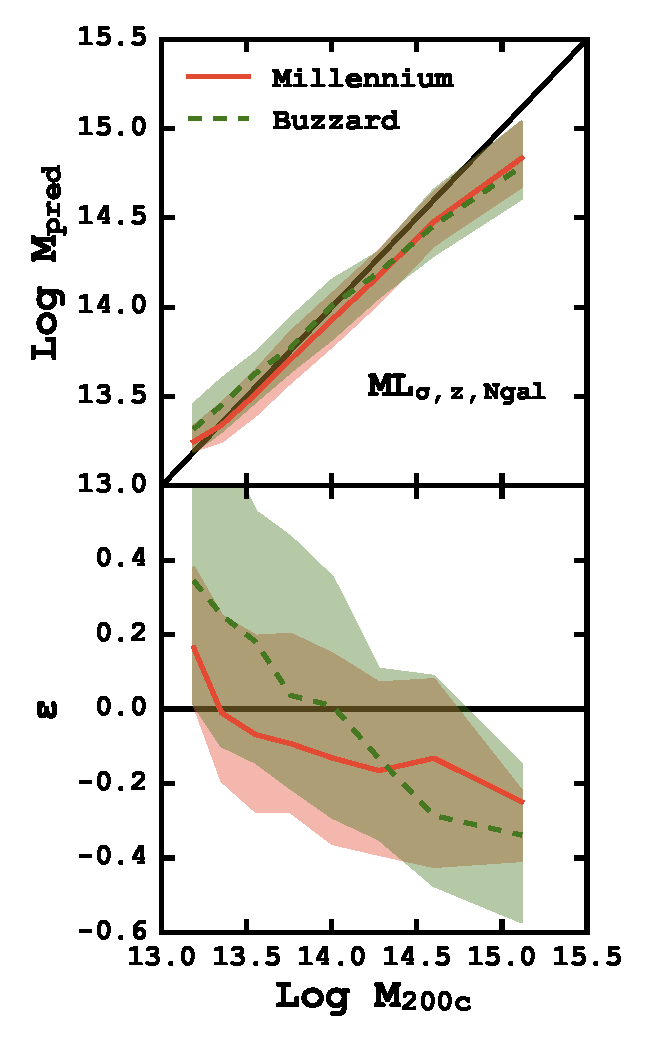
\includegraphics[width=\textwidth]{figures1/millBuzzComparison.pdf} 
	\caption{\emph{Top:} ML based cluster mass predictions for the Millennium simulation clusters where the ML method has been trained with either a subset of the Millennium clusters (solid line) or the Buzzard catalog (dashed line). The shaded areas show the 68\% scatter around the median. The solid black line shows the 1:1 relation. \emph{Bottom:} The fractional error (Equation~\ref{eq: fractional error}) also as a function of true cluster mass. The similarity of the predictions with the different training sets demonstrates how the ML method is not sensitive to the underlying cosmological assumptions.} \label{fig: mill buzz comparison} 
\end{figure}

We conduct our test in two ways. Both use the ML methods (see Section \ref{sec:machine learning method}) to predict the cluster masses of the Millennium clusters, but each test uses a different training set. First, we use the full set of clusters detected in the Buzzard catalogs (14,000 clusters with $M > 10^{11}$ \msol) to train the ML. Second, the Millennium clusters are split into training-testing samples. This provides a test case where we have different cosmological choices between the training and testing samples, and the same cosmological assumptions in both samples. 

The top panel of Figure~\ref{fig: mill buzz comparison} shows the ML predicted cluster masses for the $\sim$4000 Millennium clusters as a function of true cluster mass. The orange (Millennium) and green (Buzzard) colors indicate the two different training samples. The median (solid and dashed lines) predicted cluster masses show similar trends regardless of the training data set used. The bottom panel of Figure~\ref{fig: mill buzz comparison} shows the fraction error (Equation~\ref{eq: fractional error}) also as a function of true cluster mass. The large amount of scatter (the shaded area) in the fractional error for the Buzzard-trained predictions is due to the training set including clusters with masses below the $M = 10^{13}$ \Msol\ threshold for the Millennium clusters. This allows the ML method to predict masses which can be significantly different, whereas the Millennium training set does not include $M < 10^{13}$ \Msol\ clusters, which reduces the scatter of the predicted masses.

Based on these tests, we do not find a significant cause for concern with using trained ML methods to predict our galaxy cluster masses when the underlying cosmological choices are different. This highlights the versatility of our chosen ML method. The ML method could be further diversified by including cluster measurements from a wide range of cosmological simulations (or observations) which, in affect, marginalizes over all the cosmological assumptions further reducing the dependence.

\section{HETDEX as a Galaxy Cluster Survey at $z < 0.5$}\label{sec:discussion}

\subsection{Constraints on Cosmological Parameters}
Galaxy clusters trace the peaks in the universal matter density, often referred to as the power spectrum of matter density fluctuations or the matter power spectrum. This enables them to be sensitive probes of $\Omega_m$, the total mass ($\Omega_b + \Omega_c$) density, and $\sigma_8h^{-1}$, the normalization of the power spectrum. We constrain these parameters by the comparison of the number density of observed clusters to that predicted in cosmological models. Although, in reality, one measures $\sigma_8h^{-1}\Omega_m^q$, where the value of $q$ depends on the masses and redshifts of the halos considered.

To get a sense of how well HETDEX will be able to constrain cosmological parameters we follow the discussion of \defcitealias{Weinberg2013}{W13}\cite{Weinberg2013} (hereafter \citetalias{Weinberg2013}), and begin with a few simplifying assumptions. While sensitive to $\Omega_m$, the number density of clusters does not necessarily provide the strongest contraint, but combined with other data sets (\eg, CMB, BAO, supernovae, WL, etc.) it will constrain $\Omega_m$ to higher precision.

To estimate the error associated with a measurement of $\sigma_8h^{-1}$ (which \citetalias{Weinberg2013} refer to as $\sigma_{11,abs}$), \citetalias{Weinberg2013} consider two sources of uncertainty, the systematic uncertainties in cluster mass calibration and the statistical uncertainty in the observed number density of clusters. The authors combine these two uncertainties though (their Eq. 141):
\begin{equation}
\Delta \ln \sigma_8h^{-1}(z) \approx q(z)\times 
        \max\left[ \Delta \ln M, \alpha(z)^{-1} \Delta \ln N \right].
\label{eq:sigElapprox}
\end{equation}
where $q$ is the degeneracy exponent between $\sigma_8h^{-1}$ and $\Omega_m$, $\Delta \ln M$ is the mass scale uncertainty, $\Delta \ln N$ is the cluster statistical uncertainty, and $\alpha$ is slope of the cumulative HMF. Using the \cite{Tinker2008} HMF at $z\sim0.2$ and a limiting cluster mass of $10^{14}$ \Msol, \citetalias{Weinberg2013} estimate $q\sim0.4$, $\alpha\sim3$, and find that any cluster survey with more than 10-20 clusters is dominated by the uncertainty in the overall mass scale.

For a survey such as HETDEX, we can estimate the constraints on $\sigma_8h^{-1}$ using Equation \ref{eq:sigElapprox}. If we consider clusters with masses above $10^{14}$ \Msol\ and with Perfect knowledge observations, the lowest mass scale uncertainty (given in Table~\ref{tbl:mass scatter}) is $\Delta_{log_{10}}M \sim 0.075$ dex or about 20\%. This gives a uncertainty on $\sigma_8h^{-1}$ of 7\%. For clusters above $10^{14}$ \Msol, Survey observations constrain the masses to about 51\% which, in turn, constrains $\sigma_8h^{-1}$ to 20\%.

Because of the simplifying assumptions, and the superior quality of the data (no contamination, signal-to-noise issues, etc.), realistic expectations for HETDEX is to directly constrain $\sigma_8h^{-1}$ is not yet competitive with other methods (\eg, CMB, WL, X-ray). For example, \cite{deHaan2016} constrain $\sigma_8h^{-1}$ to $\sim5$\% using a sample of 337 SZE detected clusters from the SPT-SZE survey. For the $\sim1500$ clusters detected with Survey observations to constrain $\sigma_8h^{-1}$ and to be dominated by cluster statistics alone ($\Delta \ln N \sim N^{-1/2}$), the absolute cluster calibration would need to be better than 2.5\%. For a fully Targeted survey, about 14,000 clusters, this cluster mass calibration uncertainty reduces to $>1\%$. So while, the contraints produced by HETDEX will be larger than some other studies, the type of data provided by HETDEX will enable an independent calibration from other cluster mass measurements. This will provide important systematics checks on other studies and will ultimately improve the measurements of $\sigma_8h^{-1}$ .

\subsection{Scale and Scatter of the Richness-Cluster Mass Relation}
Large-scale optical surveys (\eg, DES and LSST) expect to detect hundreds of thousands of galaxy clusters at $z < 1$. Because they produce photometry only, a major challenge for these surveys is relating a cluster observable to the total DM mass. One promising cluster mass estimator is the optical richness \citeeg{Abell1958}. Specifically, here, we use $\lambda$, the weighted number of galaxies within a scale aperture \citeeg{Rozo2011} as calculated by the redMapper algorithm \citep{Rykoff2012}. Previous works \citeeg{Rozo2010} show that the richness correlates strongly with cluster mass on the average, but the absolute mass scale of the optical richness mass estimator and the scatter in cluster mass at fixed optical richness are imprecisely known \citep{Rykoff2012}. These systematics remain the major source of uncertainty in deriving cosmological constraints from cluster abundances and must be measured using independent methods to realize the full potential of these types of surveys.

One of the main goals of this study is to understand how well HETDEX will be able to measure the scatter in the richness-mass relationship. To this end, we choose to impose a richness-mass relation onto the clusters in the Buzzard catalogs. The true richness-mass relation could depend strongly on the number and types of environmental effects, because such effects have a strong impact on the number and types of galaxies observed in clusters \citeeg{Gunn1972,Balogh2000,White2010}. Any environmental effects included in Buzzard could potentially impact our observed richness. The imposition of an empirical richness-mass relation ensures the richness values correspond correctly to the clusters in our sample, could provide direct observational tests in the future.

We generate richnesses based on the true cluster masses, and for testing, we assume two versions of the richness-mass relationship. \cite{Farahi2016} base the relation on stacked velocity dispersions, and \cite{Simet2016} use weak lensing measurements to construct their relation. Because we are investigating HETDEX's ability to recover the overall cluster mass scale and underlying scatter in the mass-richness relationship, we use the true cluster masses perturbed by a known amount to estimate the observed richness. 

To confirm that measuring the underlying scatter is possible, after generating richness values we calculate the scatter of the cluster masses at fixed $\lambda$, $\sigma_{M|\lambda}$, by comparing the true, unperturbed cluster masses against the richness. We do recover the expected scatter, often, to well within 0.01 dex. We repeat the process with both assumed richness-mass relationships and recover the expected scatter in both instances. 

We use the lambda values generated above in combination with the $\mathrm{M}_{\sigma,z,N_{gal}}$ predicted cluster mass which have been bias corrected using the values in Table~\ref{tbl:mass bias} and denoted $\mathrm{M_{pred,corr}}$. The use of biased cluster mass predictions inhibits our ability to accurately recover any scatter in richness-mass relationship, and is discussed further below. 

Primarily, we are interested in the intrinsic scatter of the richness-mass relationship. This is because HETDEX is uniquely situated to estimate the scatter, whereas studies relying on stacked data \citeeg{Farahi2016,Simet2016} lose that information. We begin by attempting to constrain the absolute mass scale, and as part of our fitting process, we estimate the overall scatter in the relationship. In order to understand how HETDEX will constrain the absolute mass scale, we find the best fitting relation to our richness-mass data. To generate the best fitting lines, we follow the general procedure of \cite{Hogg2010}, by defining an objective function and then minimizing the loss. Our objective function is
\begin{equation}\label{eq:objectivei}
P(y_i|x_i,\sigma_{yi},m,b,\sigma) = \frac{1}{\sqrt{2\,\pi\,(\sigma_{yi}^2+\sigma^2)}}
 \,\exp\left(-\frac{[y_i - m\,x_i - b]^2}{2\,(\sigma_{yi}^2+\sigma^2)}\right)
\end{equation}
where $y_i$ is the observed cluster mass, $x_i$ is the observed richness, $\sigma_{yi}$ is the uncertainty in observed cluster mass, $m$ is the power law slope, $b$ is the overall cluster mass scale, and $\sigma$ is the intrinsic scatter between richness and cluster mass. We assume that the intrinsic scatter is constant from point to point and that all of the measurement errors are Gaussian. We convert this objective function into a likelihood by taking the product of all the individual probabilities:  
\begin{equation}\label{eq:like}
\mathscr{L} = \prod_{i=1}^N \ P(y_i|x_i,\sigma_{yi},m,b, \sigma).
\end{equation}
We again rely on MCMC samples to sample the posterior probability distribution and thus maximize the likelihood. The best fitting slope and intercept are quoted as the median value of the posterior probability distribution with 68\% error bars defined as the square root of the second moment of the same distribution.

We limit our clusters to those with $10 \leq \lambda < 130$ in our fitting analysis because above $\lambda=130$ there are too few clusters and number-counting errors dominate. Other observational studies \citeeg{Saro2015} which have lower limits on $\lambda$, so we exclude anything less than $\lambda=10$. For a richness-mass relation with an intrinsic scatter of $\langle \sigma_{M|\lambda} \rangle = 0.25$ dex, we find a best-fitting relation for the Targeted observations as
\begin{equation}
	\mathrm{Log}\ M_{200c}/\Msol = 12.46\pm0.02 + 1.07\pm0.02\ \mathrm{Log}\ \lambda
\end{equation} 
and the Survey observations as
\begin{equation}
	\mathrm{Log}\ M_{200c}/\Msol = 12.64\pm0.05 + 0.98\pm0.03\ \mathrm{Log}\ \lambda
\end{equation} 
This gives $M_{200c} = (1.45\pm0.12)\times10^{14}$ \Msol\ and $M_{200c} = (1.59\pm0.27)\times10^{14}$ \Msol\ at $\lambda=40$ for the Targeted and Survey observations respectively. In both cases, this normalization differs significantly from the $M_{200c} \approx 2.1\times10^{14} h^{-1}$ \Msol\ found in recent work \cite{Li2016, Simet2016}. If the intrinsic scatter is reduced to $\sim 0.05$ dex we recover an overall normalization of $M_{200c} = (2.14\pm0.12)\times10^{14}$ \Msol\ and $M_{200c} = (2.10\pm0.26)\times10^{14}$ for the Targeted and Survey observations at $\lambda=40$.

We also estimate the intrinsic scatter. For observations with a richness-mass relation intrinsic scatter of $\langle \sigma_{M|\lambda} \rangle = 0.25$ dex, we recover $\langle \sigma_{M|\lambda} \rangle = 0.236\pm0.003$ dex and $\langle \sigma_{M|\lambda} \rangle = 0.257\pm0.007$ dex for the Targeted and Survey observations respectively. 

%The discrepancy between the intrinsic value and the measured value is due to the uncertainties in the individual cluster mass predictions. As the prediction intervals are narrowed, the recovered intrinsic scatter approaches the true value. For example, with cluster mass prediction intervals half the size of the current intervals we measure $\langle \sigma_{M|\lambda} \rangle$ to be $\sim 0.25$ and $\sim 0.23$ dex for the two sets of observations.

\begin{figure} 
	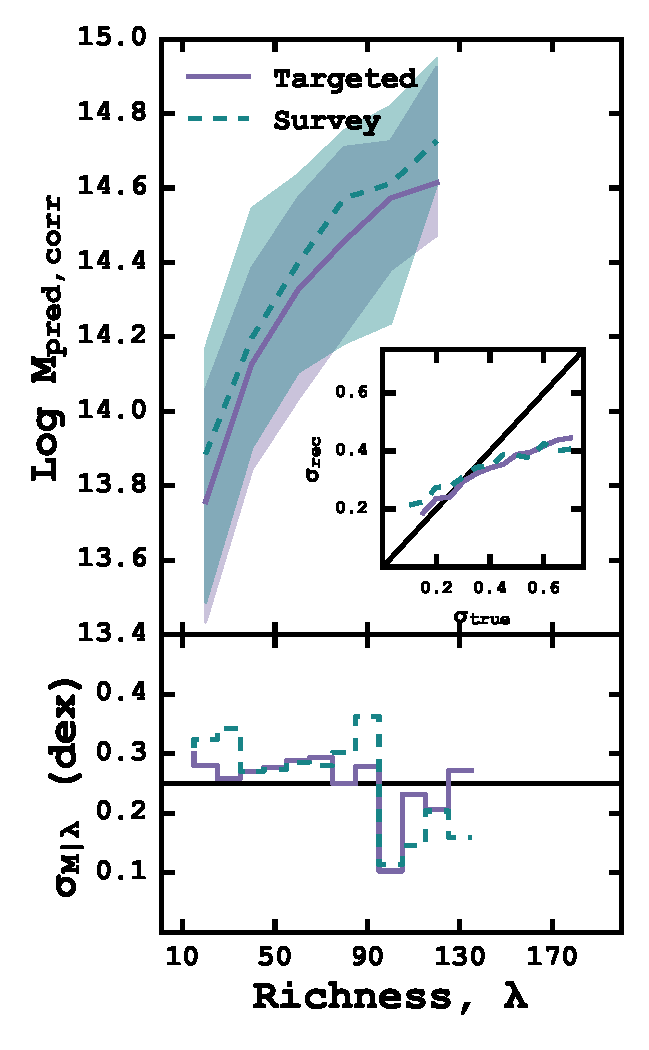
\includegraphics[width=\textwidth]{figures1/massRichness.pdf} 
	\caption{\emph{Top}: The optical richness, $\lambda$, versus the corrected predicted cluster mass. The solid, purple line is the median predicted mass for the Targeted observing, and the turquoise, dashed line is the median recovered mass for the HETDEX-like observations. The shaded regions represent the 68\% scatter around the median values. \emph{Bottom}: The scatter in the relation at fixed richness. The solid black line shows the intrinsic scatter of $\sigma_{true}=0.25$ dex. Color coding is the same as the top panel. \emph{Inset}: The evolution of the intrinsic scatter versus the average recovered scatter, $\sigma_{rec}$.} \label{fig:mass richness} 
\end{figure}

Figure \ref{fig:mass richness} summarizes the main results of this investigation. The top panel shows the generated optical richness, $\lambda$, versus the predicted cluster mass. The cluster masses are the $\mathrm{ML}_{\sigma, z, N_{gal}}$ based and correspond to the Targeted and Survey observation strategies. The bottom panel of Figure \ref{fig:mass richness} shows the scatter in the predicted cluster masses at fixed richness, $\sigma_{M|\lambda}$. The solid line represents the intrinsic amount of scatter added to the masses. The cluster masses are binned in increasing ten richness intervals ($10-20$, $20-30$, etc.). The inset upper panel shows the intrinsic scatter versus the recovered average scatter at fixed richness, $\langle \sigma_{M|\lambda} \rangle$ and illustrates how well the two observation strategies recover the intrinsic scatter. 

We find that we are able to accurately recover an average intrinsic scatter of $0.2 <\langle \sigma_{M|\lambda} \rangle <0.3$ dex, finding $\langle \sigma_{M|\lambda} \rangle = 0.257\pm0.007$ at $\sigma_{true} = 0.25$ with Survey observations. This is very promising as other observational studies have estimated the intrinsic scatter of real clusters to be $\sim0.25$ dex \citeeg{Rozo2014, Rozo2015}. As the intrinsic scatter increases or decreases, we fail to recover the scatter as accurately.

For the richness range $10 \leq \lambda < 130$ the intrinsic scatter in between the $\mathrm{M_{pred,corr}}$ predicted cluster masses and the true cluster mass (the basis of our richnesses) is $\sim0.15$ dex for Targeted observations and $\sim0.20$ dex for Survey observations. This forms an effective floor on the amount of scatter we are able to recover from our fitting process. As we reduce the overall scatter in our cluster mass recovery, this floor will lower. We underestimate the scatter in high intrinsic scatter relations because any residual bias remaining in the predicted clusters masses after correction reduces the observed scatter. Because the bias subtraction when creating $\mathrm{M_{pred,corr}}$ subtracts the mean bias, we are left with a small amount of residual bias, lowering the measured scatter for high scatter relationships.

\section{Summary}\label{sec:summary}
Here, we present detailed simulations of the upcoming HETDEX survey's applicability to the detection and total mass measurement of galaxy clusters. Using mock galaxy catalogs and HETDEX-like observational strategies and limits, we observe our simulated sky, estimate the number of clusters observed, and derive basic cluster parameters, redshift, line-of-sight velocity dispersion (LOSVD). Using a traditional power law-based, velocity dispersion, scaling relation along with more advanced probability and machine learning (ML) techniques, we estimate each cluster's total mass. We discuss each cluster mass estimate's precision, and discuss HETDEX's ability to constrain the cosmological parameter $\sigma_8 h^{-1}$ based on those predicted cluster masses. In addition, we comment on how HETDEX may improve current and future photometric large-area sky surveys' cluster mass estimates derived from optical richness.

Our main conclusions are the following:
\begin{enumerate}
	\item After considering HETDEX's observational limits, we find 14,189 clusters with at least five cluster members in the HETDEX survey volume. Of those, 1,760 clusters are detected with HETDEX-like survey observations. The number of cluster members recovered with Survey observations is almost exactly 4.5 times fewer than a fully Targeted survey, across both a wide range of redshifts and cluster masses.
	
	\item We find a traditional power law conversion from LOSVD to cluster mass predicts the true cluster mass with little bias or scatter for clusters Log M/\Msol\ $=14.5$ and above. Below this mass the bias and scatter rapidly increases. In contrast, the probability based and ML based cluster mass estimators are able to predict cluster mass with similar or smaller scatter across all cluster masses. The scatter further decreases when the probability based and ML estimators are combined with other cluster observables besides the LOSVD. For HETDEX-like observations and clusters with $13 < \mathrm{Log}\, M/\Msol <14.5$, we find the $\mathrm{ML}_{\sigma, z, N_{gal}}$ method results in the smallest scatter. Below Log M/\Msol\ $=13$ no method with Survey observations gives a bias of less than 50\%. For the highest mass clusters the power law method gives the lowest bias and scatter. In short, no single method is superior in all regards. The technique should be chosen to minimize the desired systematic, but we find $\mathrm{ML}_{\sigma, z, N_{gal}}$ provides the best performance across the large range of cluster masses, and observation strategies.
	
	\item In general, we find that the measured scatter of cluster masses decreases when considering Targeted versus Survey observations. Clusters at all masses can benefit from targeted follow-up observations, although the accuracy gain will be smaller than can be achieved from cluster mass prediction method changes. Targeted follow-up observations reduces the measured scatter by $\sim10\%$ when comparing like recovery methods.
	
	\item The $\sim51\%$ cluster mass accuracy of Survey observations places approximately a 20\% constraint on $\sigma_8 h^{-1}$. This can be tightened to approximately 12\% with follow-up targeted observations. Most importantly, the observations from HETDEX will provide systematics checks on other studies, ultimately improving all future measurements of $\sigma_8 h^{-1}$
	
	\item HETDEX will be able to place important, independent constraints on the amount of scatter in the optical richness-mass relationship. It will to a less extent constrain the overall normalization of the relation. This should provide an important tool in the calibration of large-area sky surveys which rely on photometric data only to estimate cluster masses.
\end{enumerate}

It is the author's hope that this work may be useful to others when conducting their own research. Because this work relies heavily on (often) complex data analysis, and in order to promote transparency and reproducible science, we provide all of the code used to conduct this study at https://github.com/boada/desCluster. Regrettably, large file size prevents including the source data with the analysis routines. The authors are happy to provide them, if requested.

